\chapter{Multigrid Methods}

\section{Introduction}
In the previous chapter, we encountered Pressure Poisson's Equation (PPE) and used Successive Over Relaxation (SOR) method to reach the solution for pressure.
However, we concluded that SOR has very slow convergence and faster methods should be used to solve the PPE.  Fast Poisson solvers use advanced techniques, 
such as discrete Fast Fourier transform or cyclic reduction, multigrid methods and iterative Krylov-subspace methods. \par
Developed in late eighties (\cite{wesseling1995introduction},\cite{briggs2000multigrid}), Multigrid methods has been used by many authors to solve PPE. We first discuss the characteristics of 
classic iterative methods and then show how the concepts from the analysis can be used to accelerate the convergence, and subsequently state the algorithm which we will 
implement in the solver to solve the PPE. The PPE has to be solved while solving the Navier-Stokes equation which is the most expensive 
part of the solution as it takes most of the time. Hence there is a need to solve this equation efficiently.Multigrid method has been developed for serial processor.

\section{General Iterative Methods}

As the discretised form of Poisson's equation has a system of linear algebric equations. We consider a one dimensional Laplace equation as it is easier to study
analytically. 
\begin{equation}
\frac{d^2u}{dx^2} = 0
\end{equation}
having boundary conditions,
$u(0)=0$ and $u(L) = 0$, which has the exact solution simply $u(x) = 0$. We now look into a numerical method to get the solution of this equation. First we
discretise the differential equation and get algebric equations.
\begin{equation}
\begin{align}
 \frac{u_{i+1}-2u_{i}+u_{i-1}}{h^2} &=& 0 \\
 \text{or,}\quad u_{i+1}-2u_{i}+u_{i-1} &=& 0 \\
 \text{of form,}\quad Ax&=&b
 \end{align}
 \label{E1}
\end{equation}

But the iterative methods don't solve $x = A^{-1} b$, rather the problem is formulated as $x = Px + Q$. These generally differ in the forms of $P$ and $Q$. 
For Gauss-Seidel method, we can split the operator A, as shown in Fig.\ref{Fig:matrix} in strictly lower, diagonal and strictly upper parts i.e. $A = L + D +U$. 
\begin{figure}
 \centering
 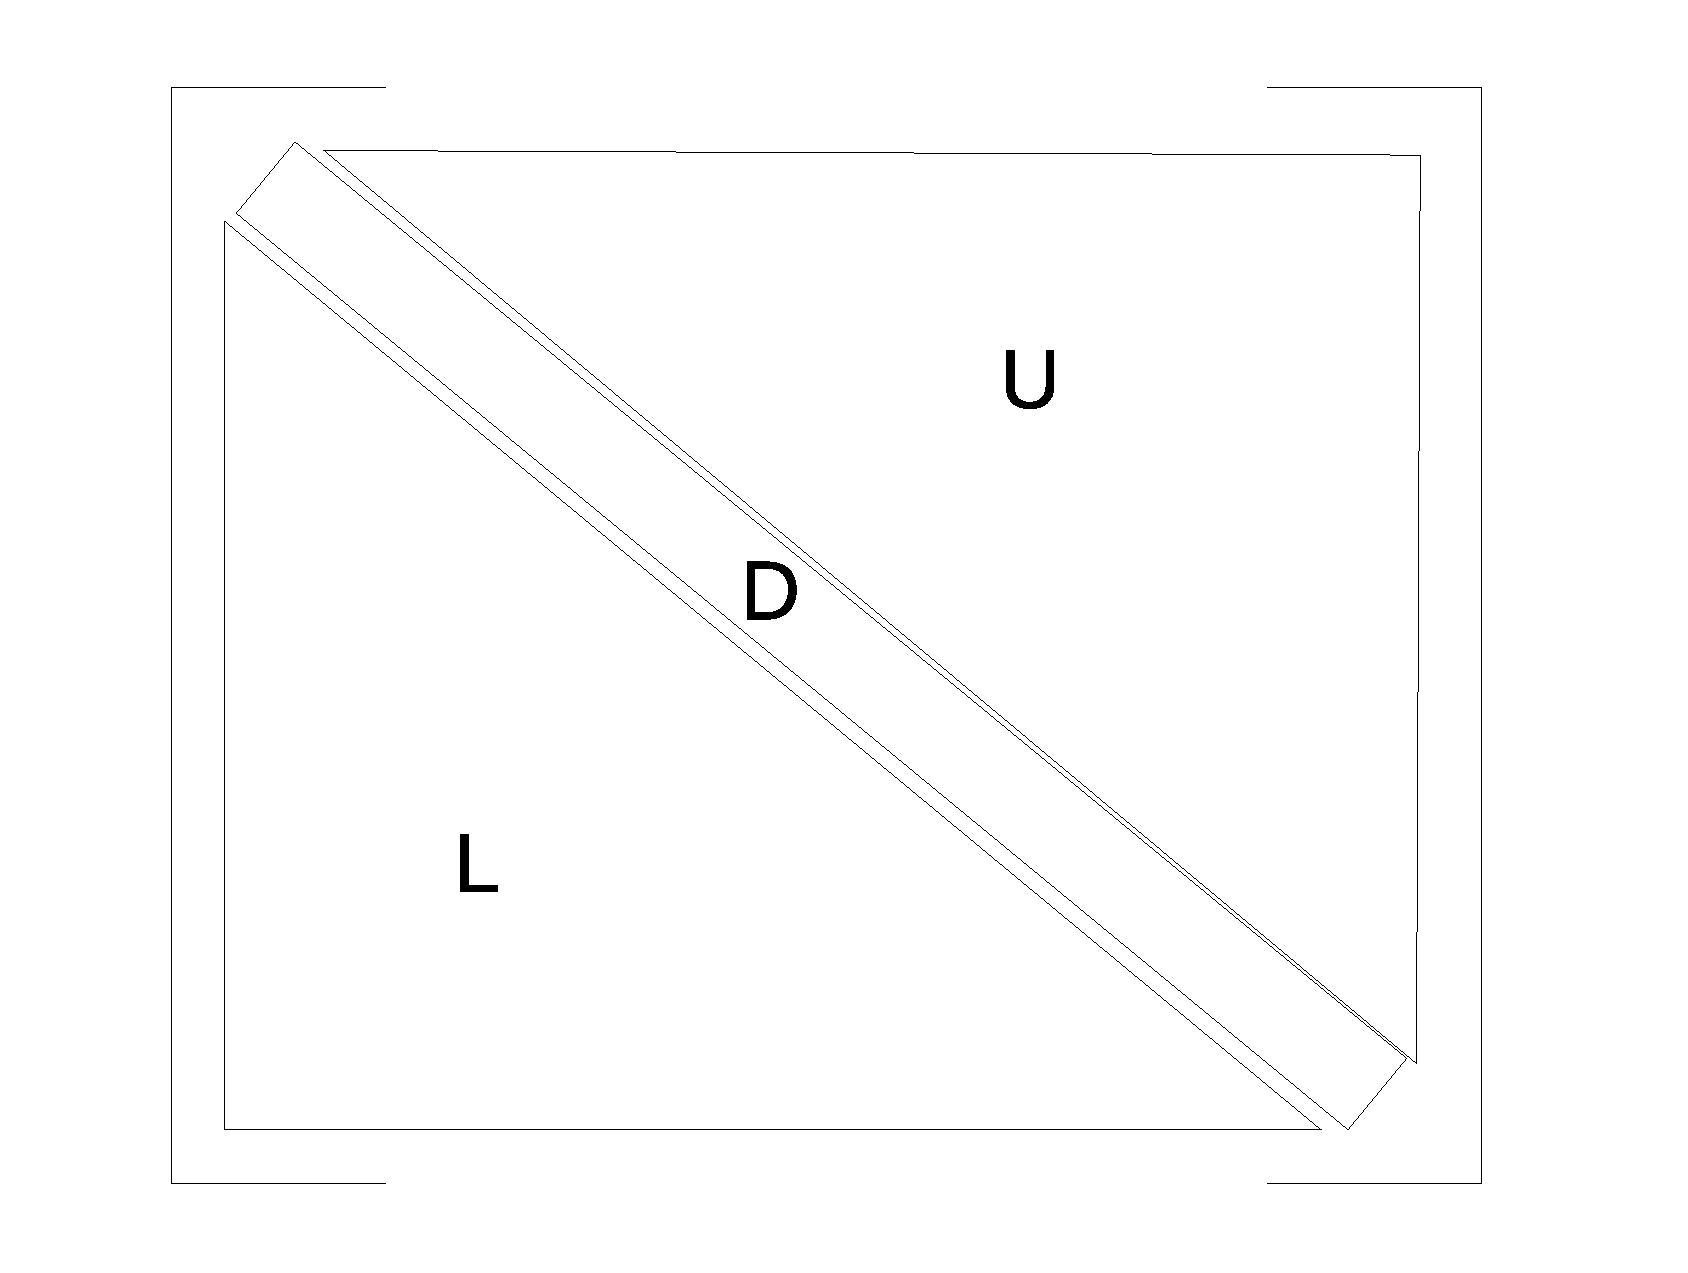
\includegraphics[scale=0.2]{mat-A.eps}
 \caption{The matrix A}
 \label{Fig:matrix}
\end{figure}

\begin{equation}
 \begin{align}
  (D +  L + U)x &= b \\
  (D+L)x &= -Ux + b \\
  x^{j+1} &= (D+L)^{-1}(-U) x^j + (D+L)^{-1}b
 \end{align}
\label{E2}
\end{equation}
\vspace{1cm}
From \ref{E2} we can see that $P = (D+L)^{-1}(-U) $ and $ Q = (D+L)^{-1} $. \par

For problem \ref{E1}, the error is defined as $e^j = u^e - u^j$, where $e^j$ is
the the error and $u^j$ is the value of $u$ at j\textsuperscript{th} iteration. The exact answer to the problem is known $u^e = 0$ at all x,
hence the error, is simply  $e^j =  - u^j$. \par
We can now discuss the behavior of Gauss-Seidel method by starting with arbitrary initial guesses. To find the characteristics for different error profiles, we solve the 
problem with initial guesses given by, 
\begin{equation}
 u_i = sin\left(\frac{k\pi x_i}{L}\right)
 \label{E3}
\end{equation}

\begin{figure}
 \centering
 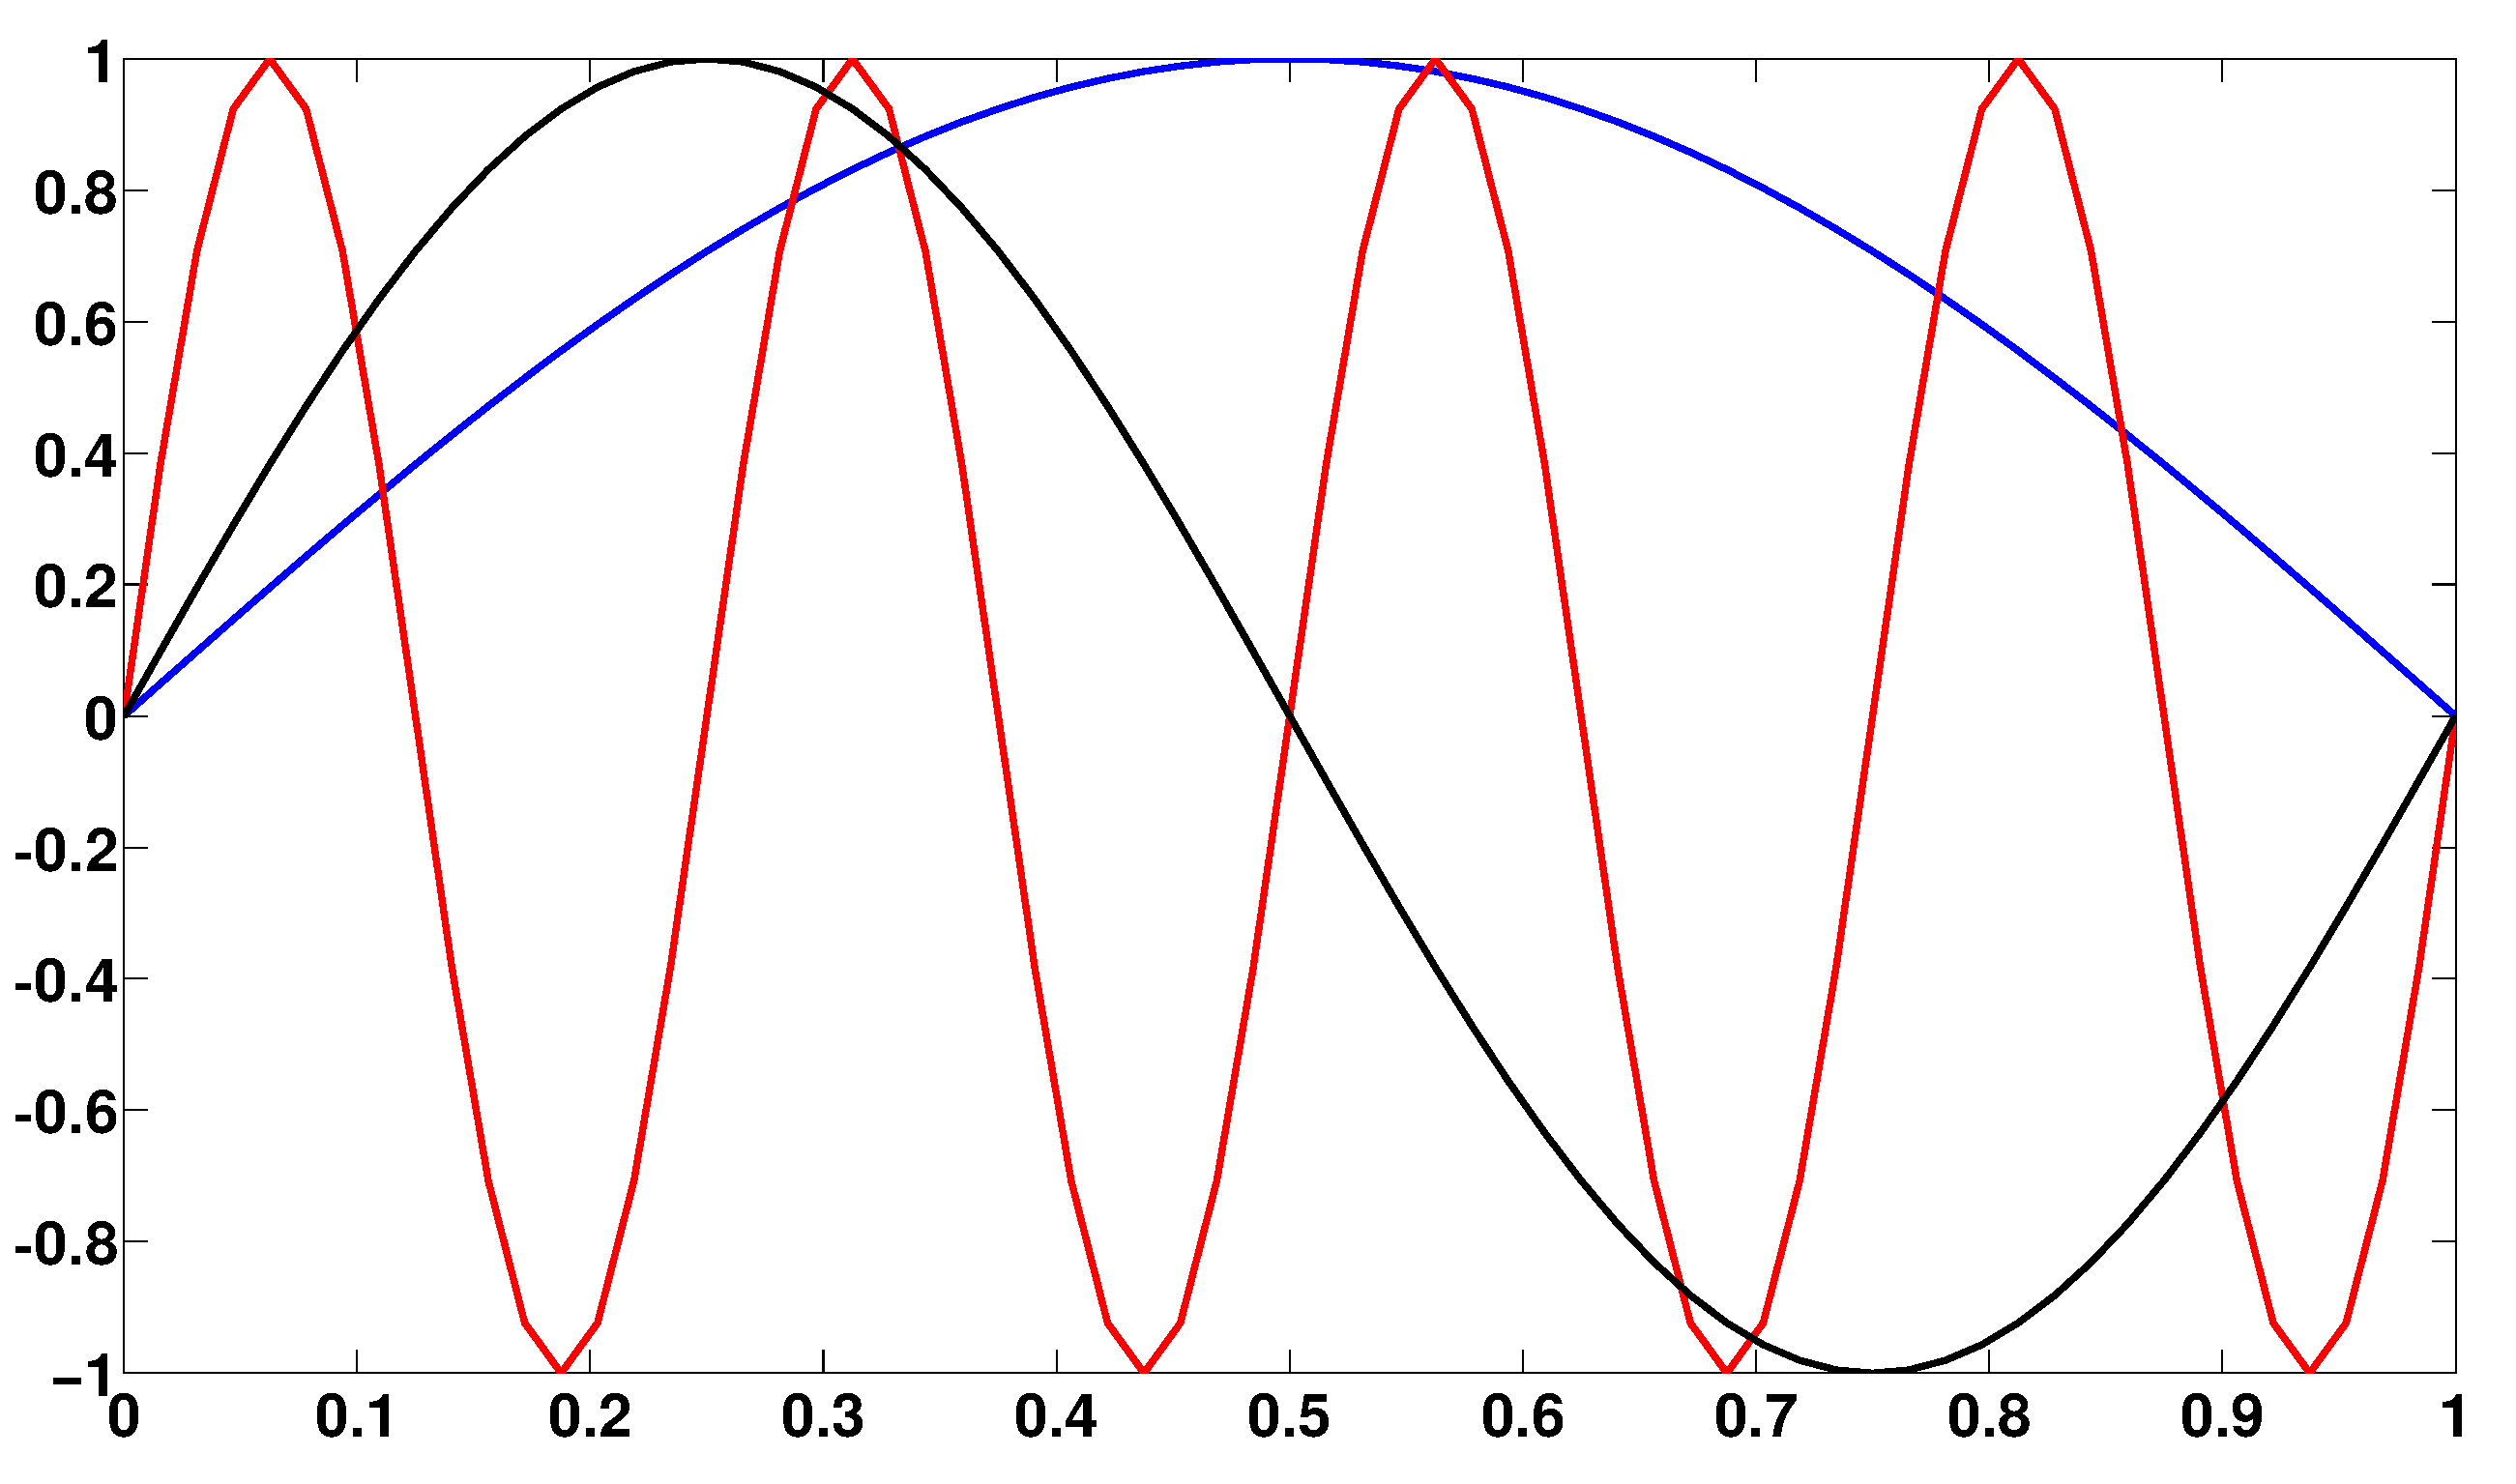
\includegraphics[scale=0.2]{Fourier_modes.eps}
 \caption{Fourier modes}
 \label{Fig:modes}
\end{figure}

In Eq. \ref{E3}, Fourier modes and k is the wavenumber. Fig. \ref{Fig:modes} shows the modes over the domain for k=1, 2 and 8. We can see for low values of k the error is 
smooth and for higher wavenumbers the profiles are oscillatory.

\begin{figure}
\centering
  \subfloat[k=1 ]{%
      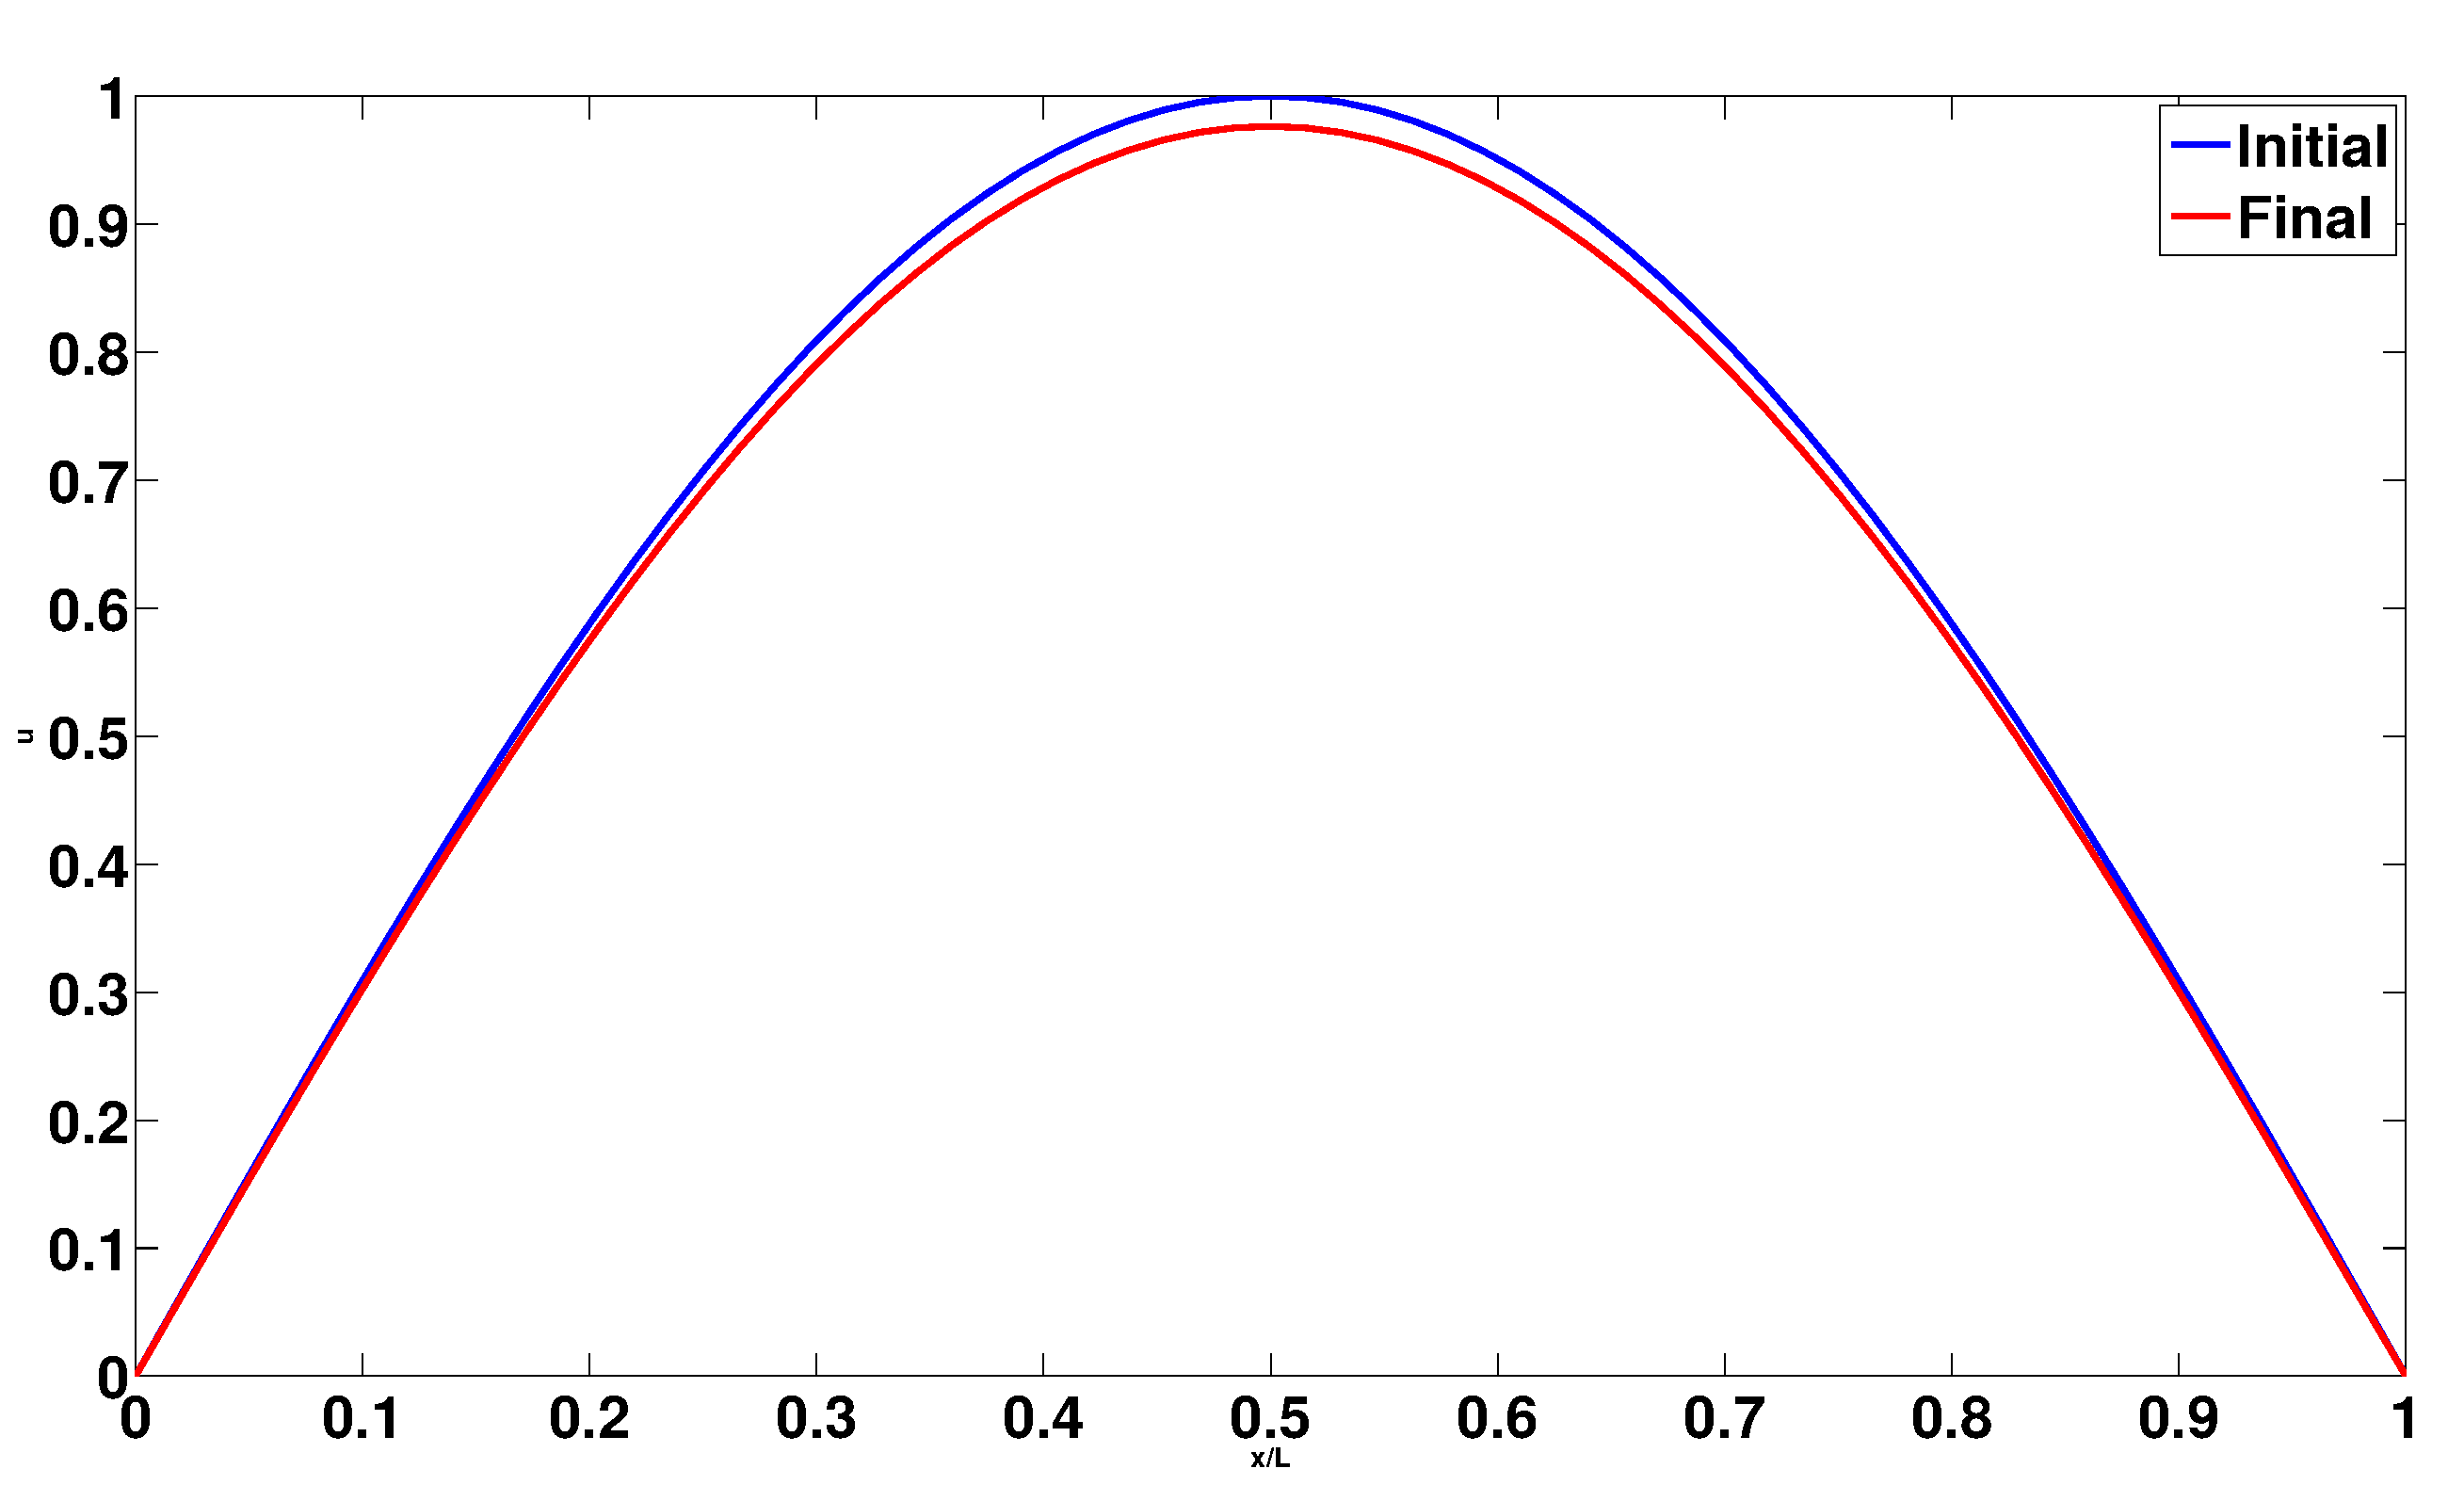
\includegraphics[width=0.5\textwidth]{k1.eps}
      }	
 \subfloat[k=2 ]{%
      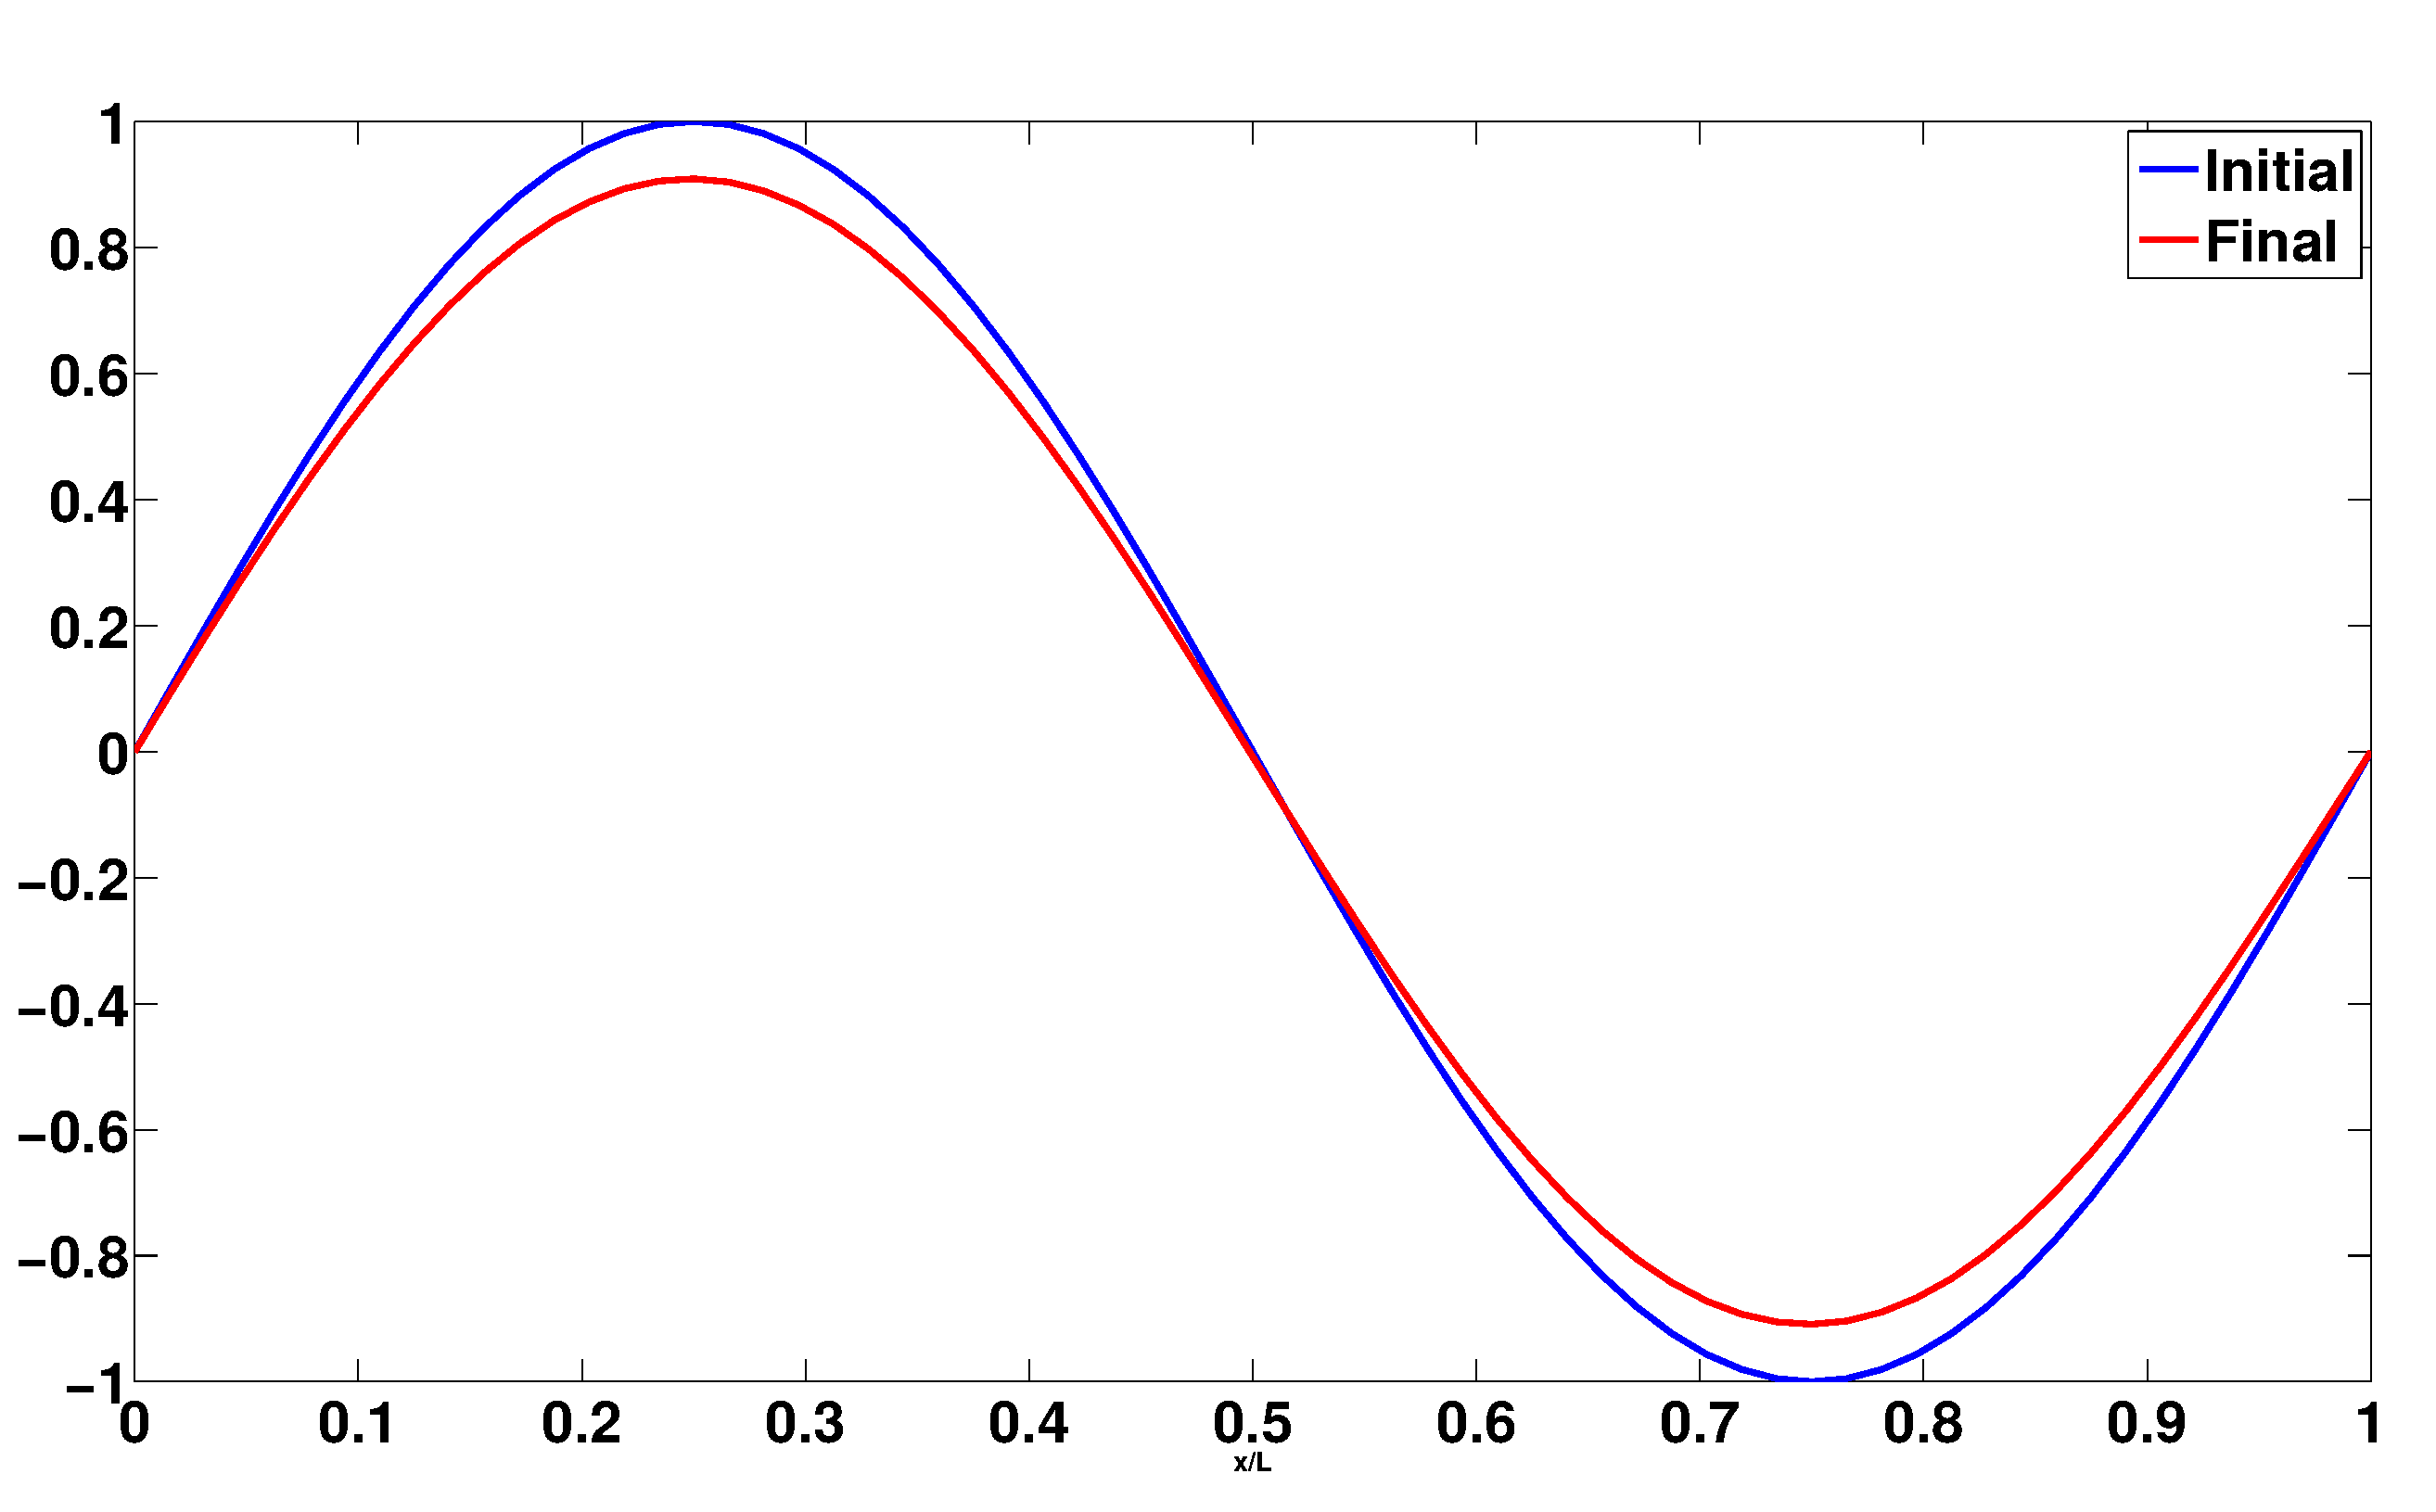
\includegraphics[width=0.5\textwidth]{k2.eps}
      }\\
  \subfloat[k=3 ]{%
      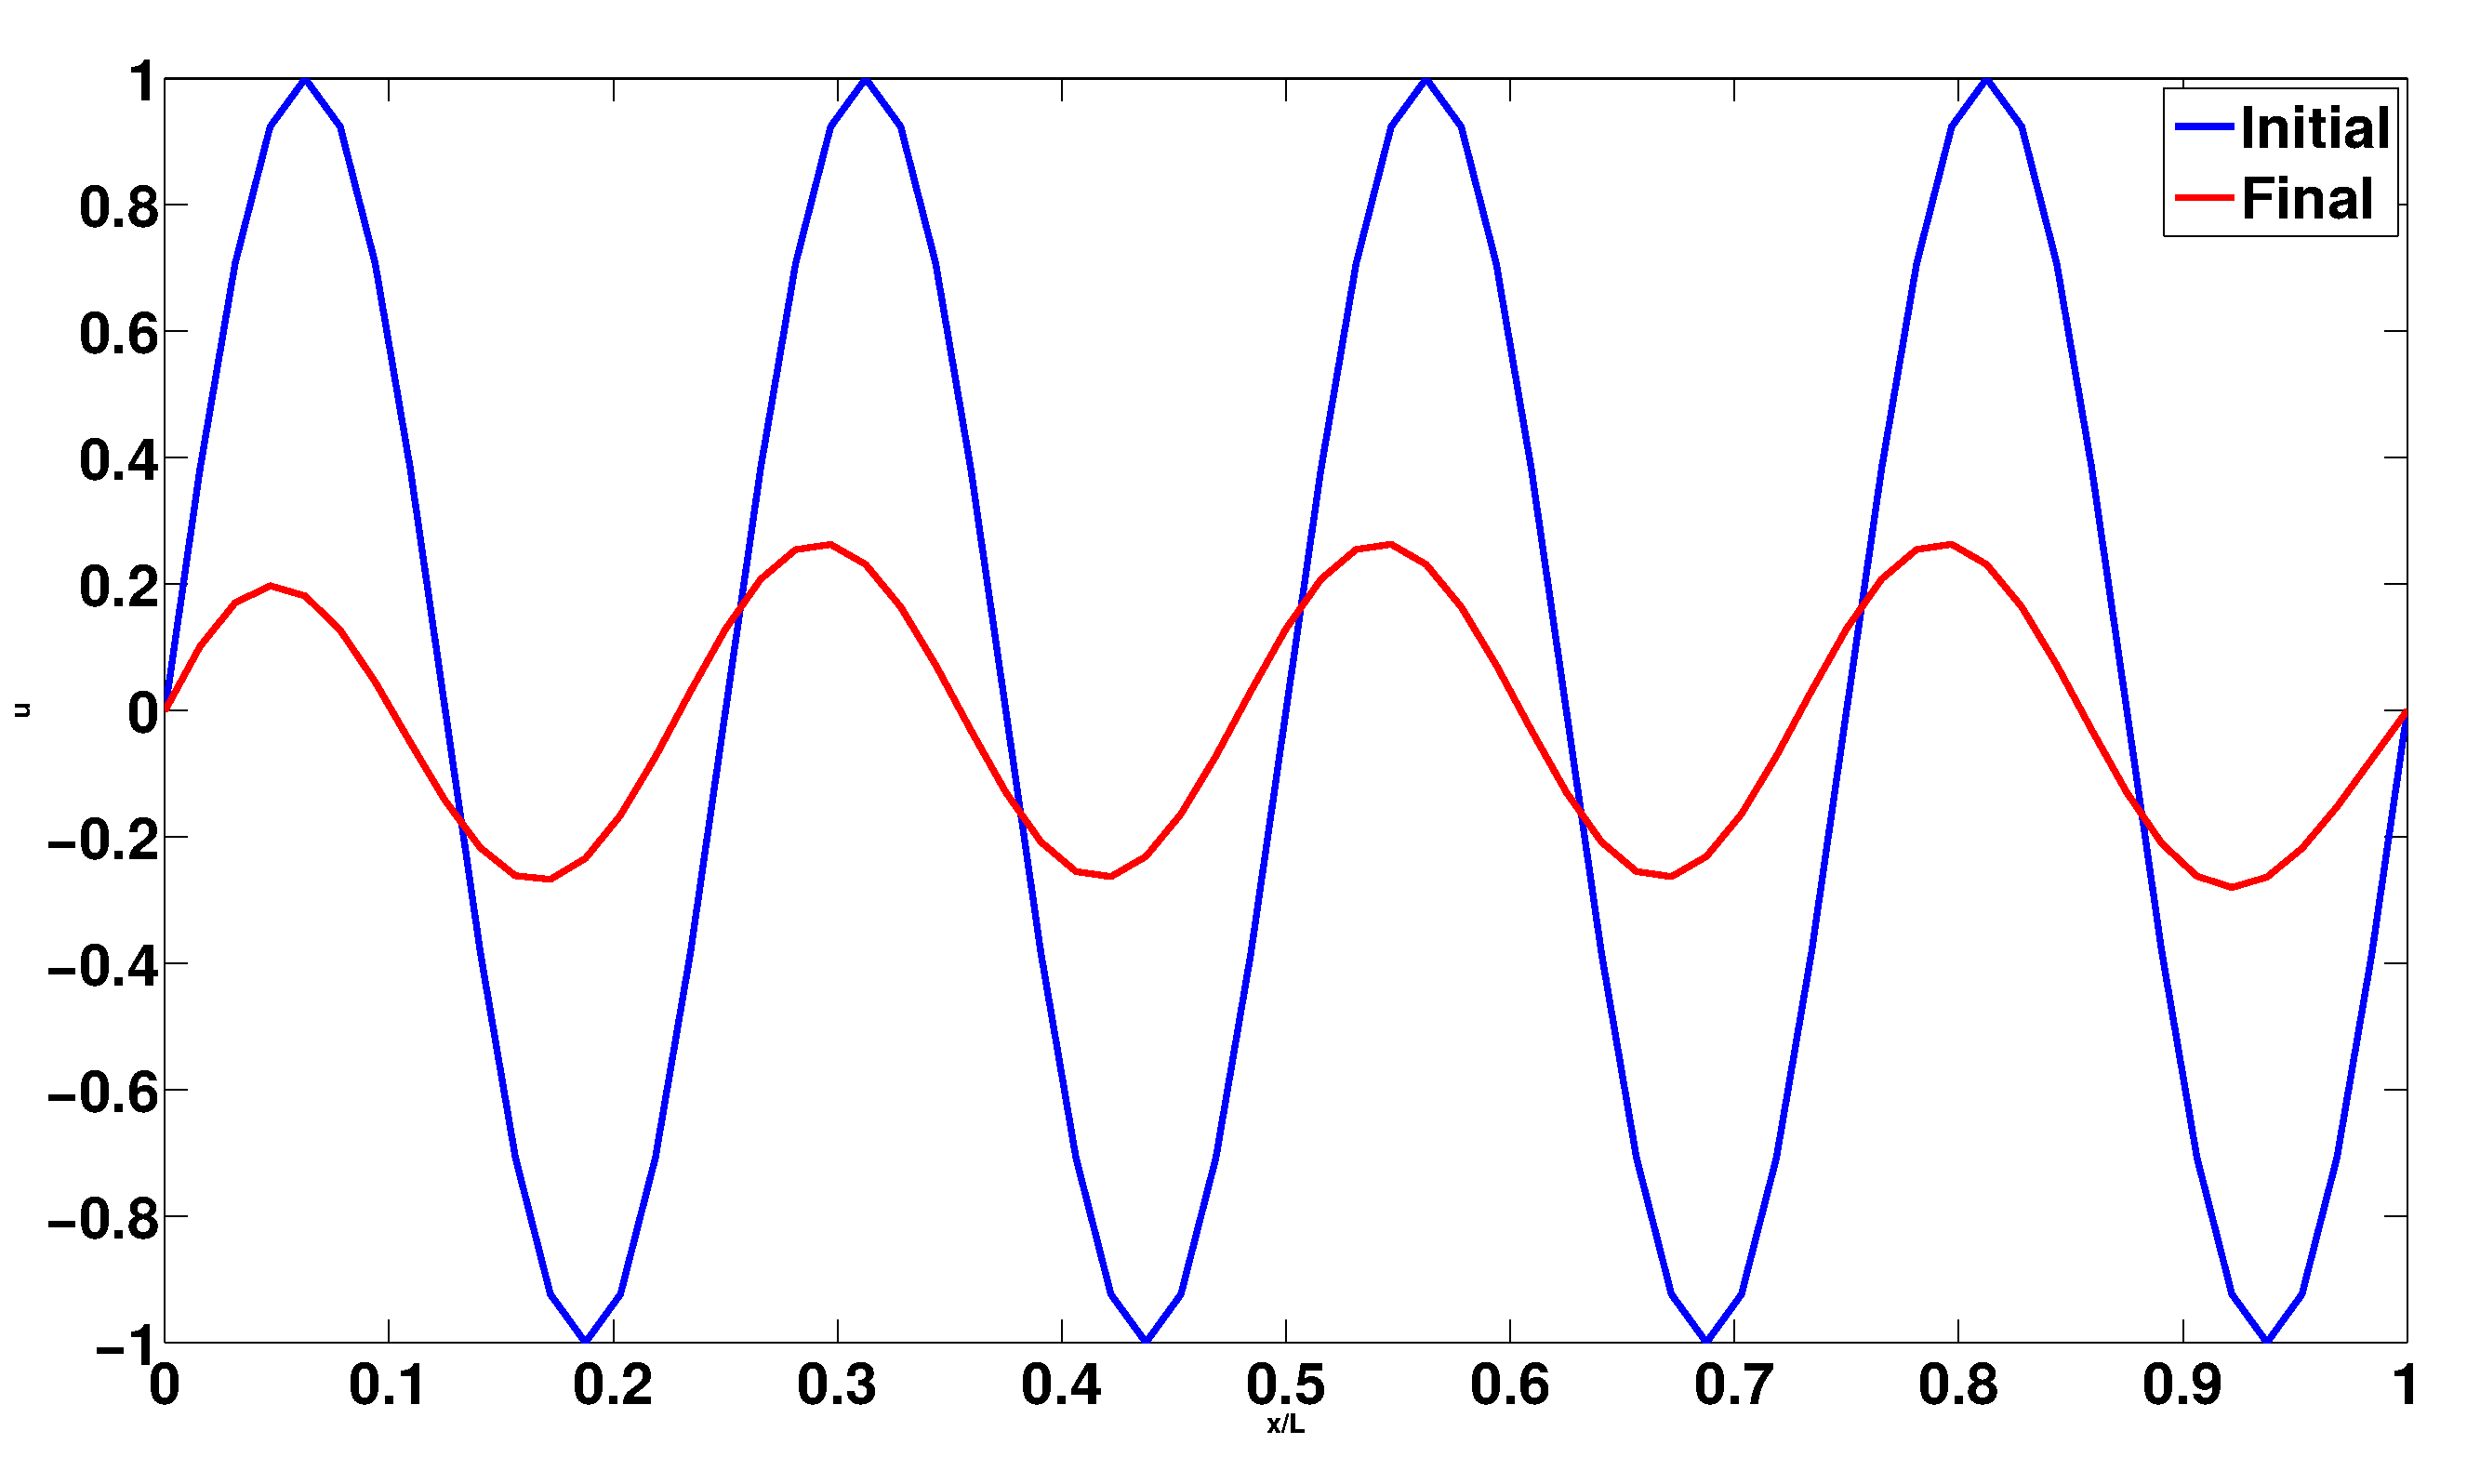
\includegraphics[width=0.5\textwidth]{k8.eps}
      }	

 \caption{Profile after 10 Gauss-Siedel iterations, Blue - Inital guess, Orange - After 10 iterations}
 \label{Fig:modes_iter}
\end{figure}

In Fig. \ref{Fig:modes_iter}, we can see for a given number of iterations the method converges faster for higher values of wavenumber in the error. 
To know the dependence of wavenumber on the convergence we have to analyse the characteristics of Gauss-Sidel method.

\subsection{Convergence analysis of Gauss-Siedel method}

We know that while approaching to the solution the error approaches to zero. We might want to look how the error decimates with respect to iterations. 
\begin{equation}
 \begin{align}
 e^n = P^n e^0
 \end{align}
 \label{E4}
\end{equation}

Now, if we expand $e^0$ in eigen basis of $P$, we get,
\begin{equation}
 e^0 = \Sigma C_k v_k
\end{equation}
where $C_k$ are the components of $e^0$ in eigen basis of and $v_k$ are eigenvectors of iteration operator $P$. We know that $P$ in its eigenbasis 
will only strech or contract the components when operated on a vector (here $e^0$) by corresponding eigenvalues $\lambda$. Hence, \ref{E4} can be expressed as,

\begin{equation}
 e^n = \Sigma \lambda^n_k C_k v_k
 \label{E5}
\end{equation}

From \ref{E5}, it can be seen that largest value of $|\lambda_k|$ should be less than 1, for the error to approach zero in successive iterations i.e. for convergence. This value is 
known as the spectral radius of the iteration matrix $P$. It can also be concluded from here that the smaller the spectral radius faster the convergence. We have observed in the
previous section that there is faster convergence for high wavenumber errors and we know that convergence is directly affected by the eigenvalues of the $P$ operator. We now look
what is the relation between the wavenumber and the eigenvalues of $P$. \par

The eigenvalues of Jacobi iteration operator is given by,
\begin{equation}
 \lambda_k = 1- sin^2\left(\frac{k\pi}{2N}\right) \hspace{1cm}\text{k = 1,2,...N}
 \label{E6}
\end{equation}

\begin{figure}
 \centering
 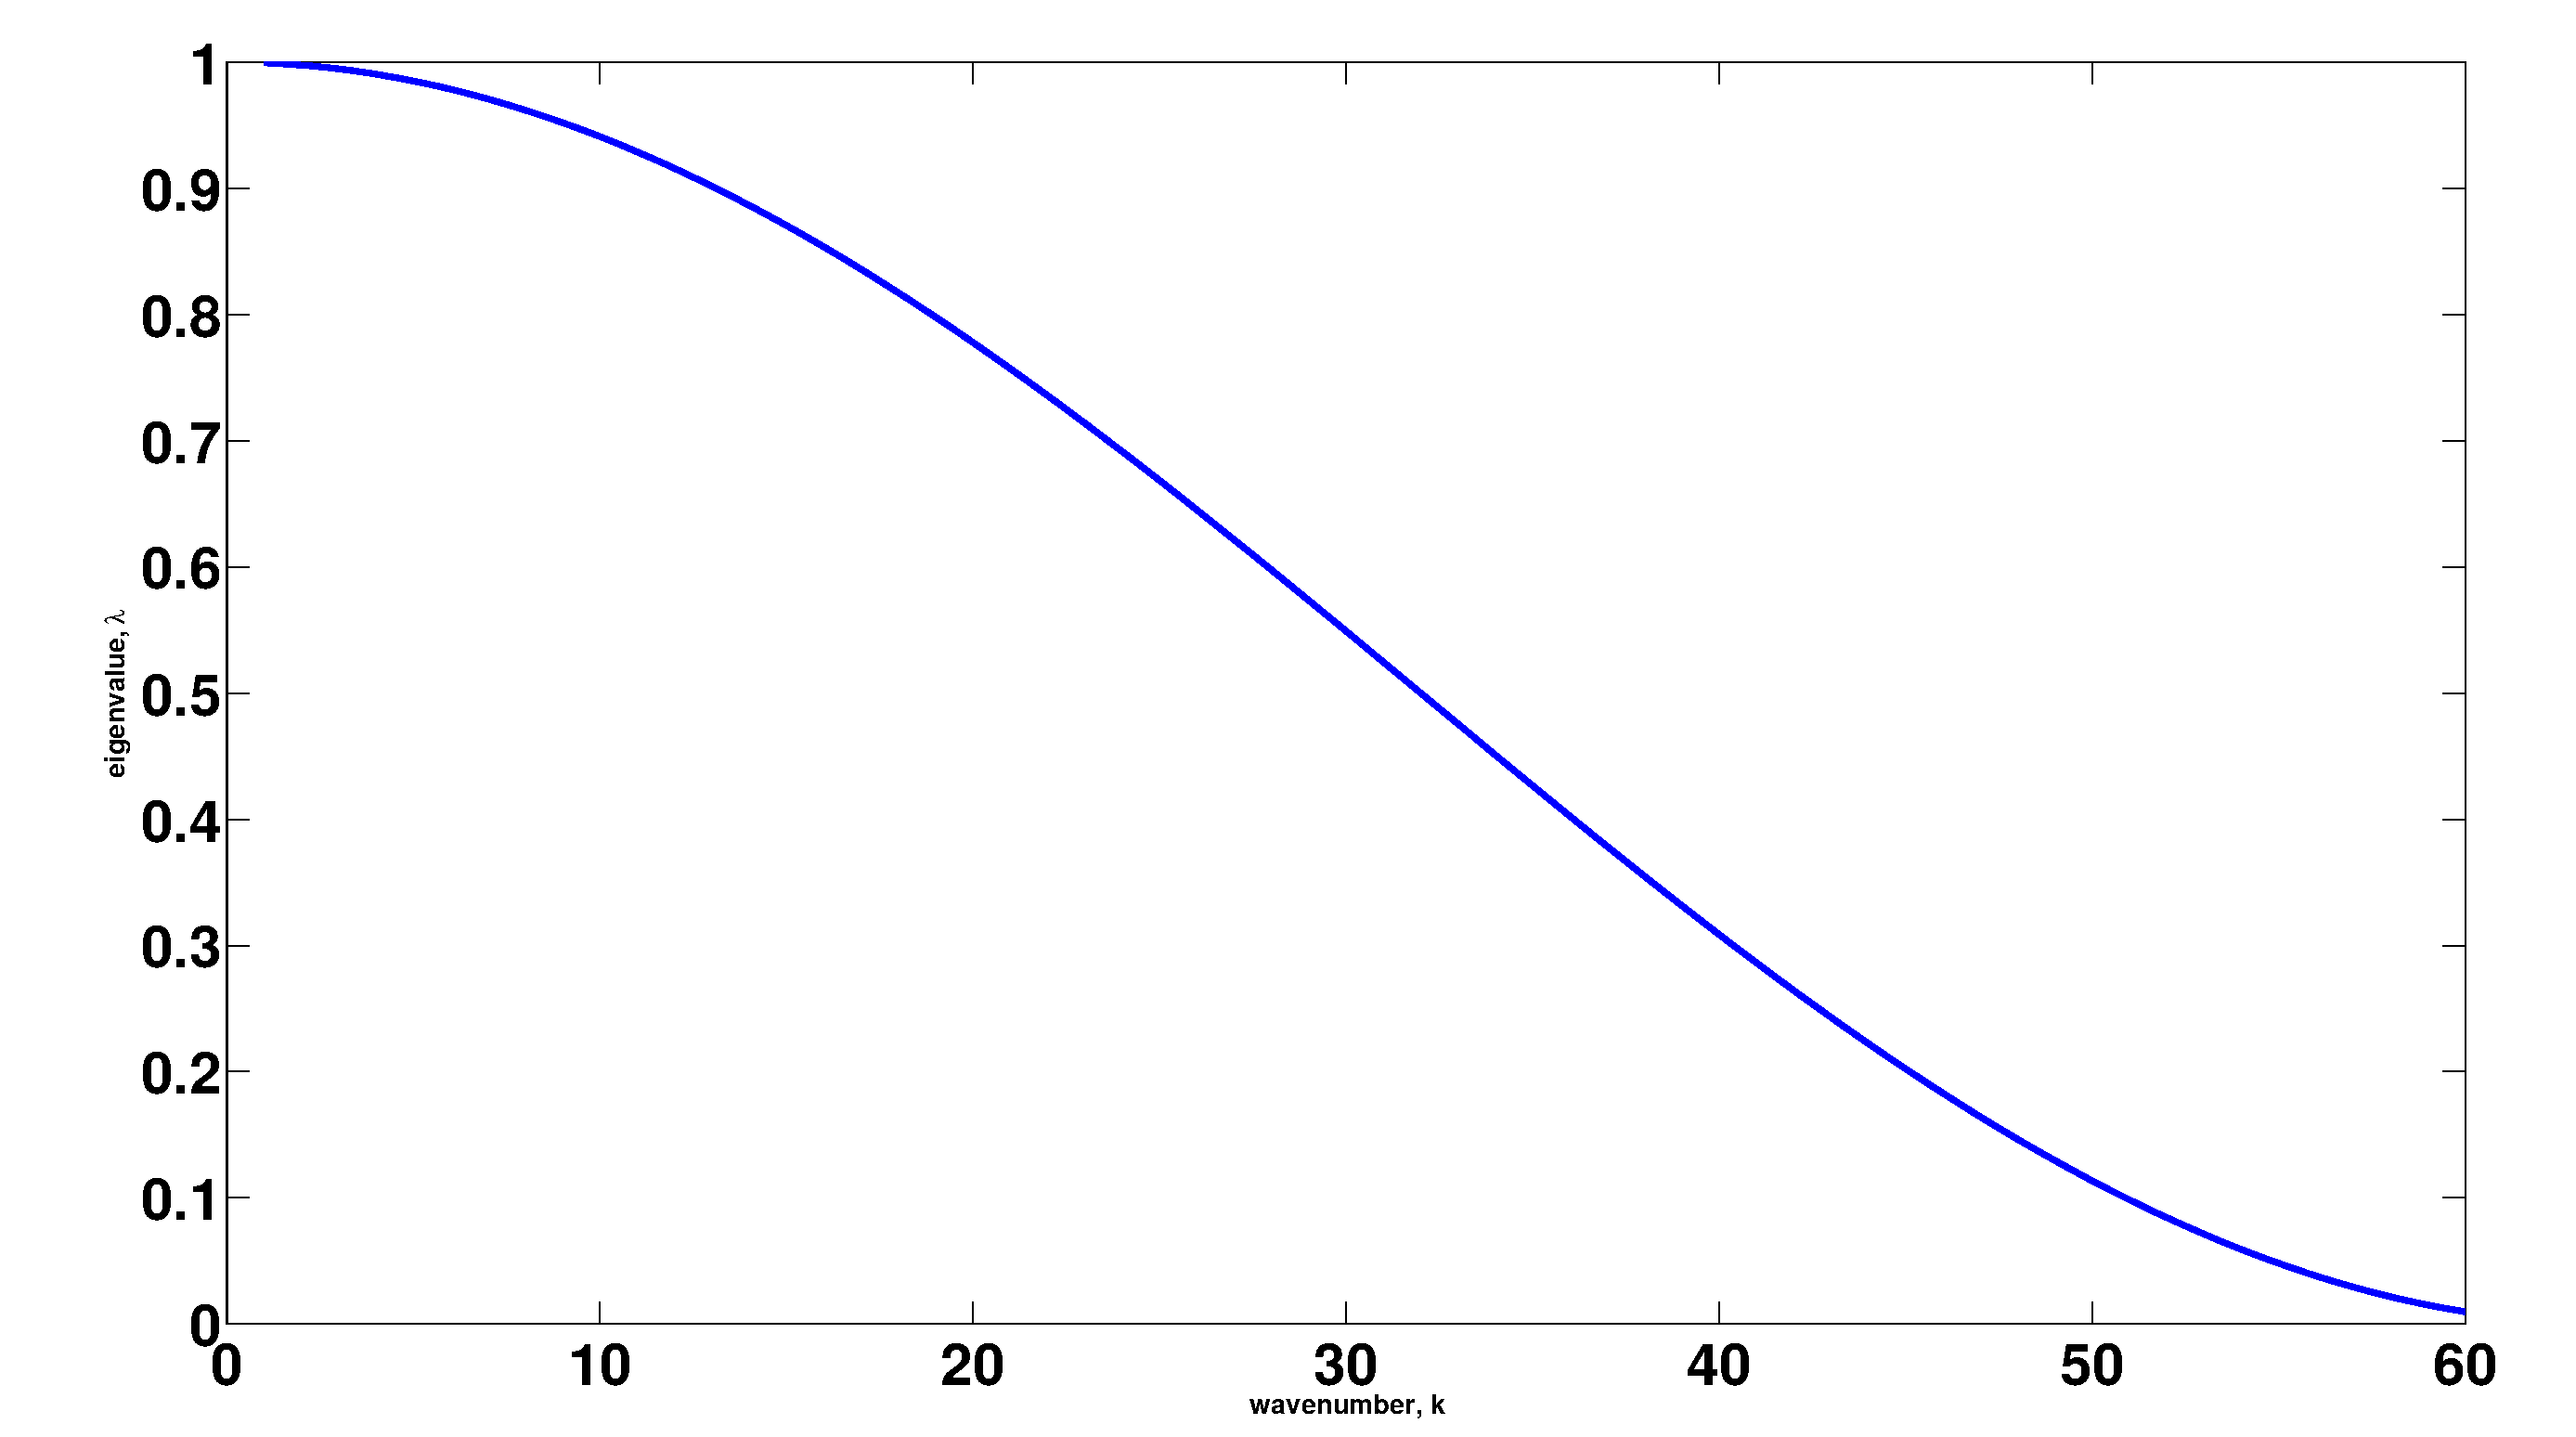
\includegraphics[scale=0.2]{eigen_vs_k.eps}
\caption{Eigenvalues$\lambda$ with respect to k}
 \label{Fig:eig_vs_k}
\end{figure}

where N is the number of nodes in the grid. From \ref{E6} we plot $\lambda$ vs k in \ref{Fig:eig_vs_k}, and we can now understand reasons for the results in previous section i.e.
the eigenvalue is low for high wavenumber modes and hence we found faster convergence for high wavenumbers.  In practical problems we don't have the solution, we need to find it and most of the times it is not even possible to give a good guess. Most
of the times we start with zero values of the variable to be calculated. Hence when we start with an arbitrary guess and it can
have errors of many wavenumbers. With this argument we cannot do much about increasing the wavenumber or the oscillatory behavior of the error.
But we can again look at \ref{E6}, the convergence depends on low values of $\lambda$, but it is not entirely dependent on wavenumber k but the ratio $\frac{k}{N}$ 
( See Fig. \ref{Fig:eig_vs_k-N} ).
For a given wavenumber $k =1$, for which convergence is low, See Fig. \ref{Fig:eig_vs_N} it can be said that low wavenumber component will converge faster on coarser grids.
This result lays down the foundation for multigrid methods. In literature we can find many variants of multigrid methods but the prime reason is buried in the dependence of eigenvalues
of the iteration operator on grid size. 


\begin{figure}
 \centering
 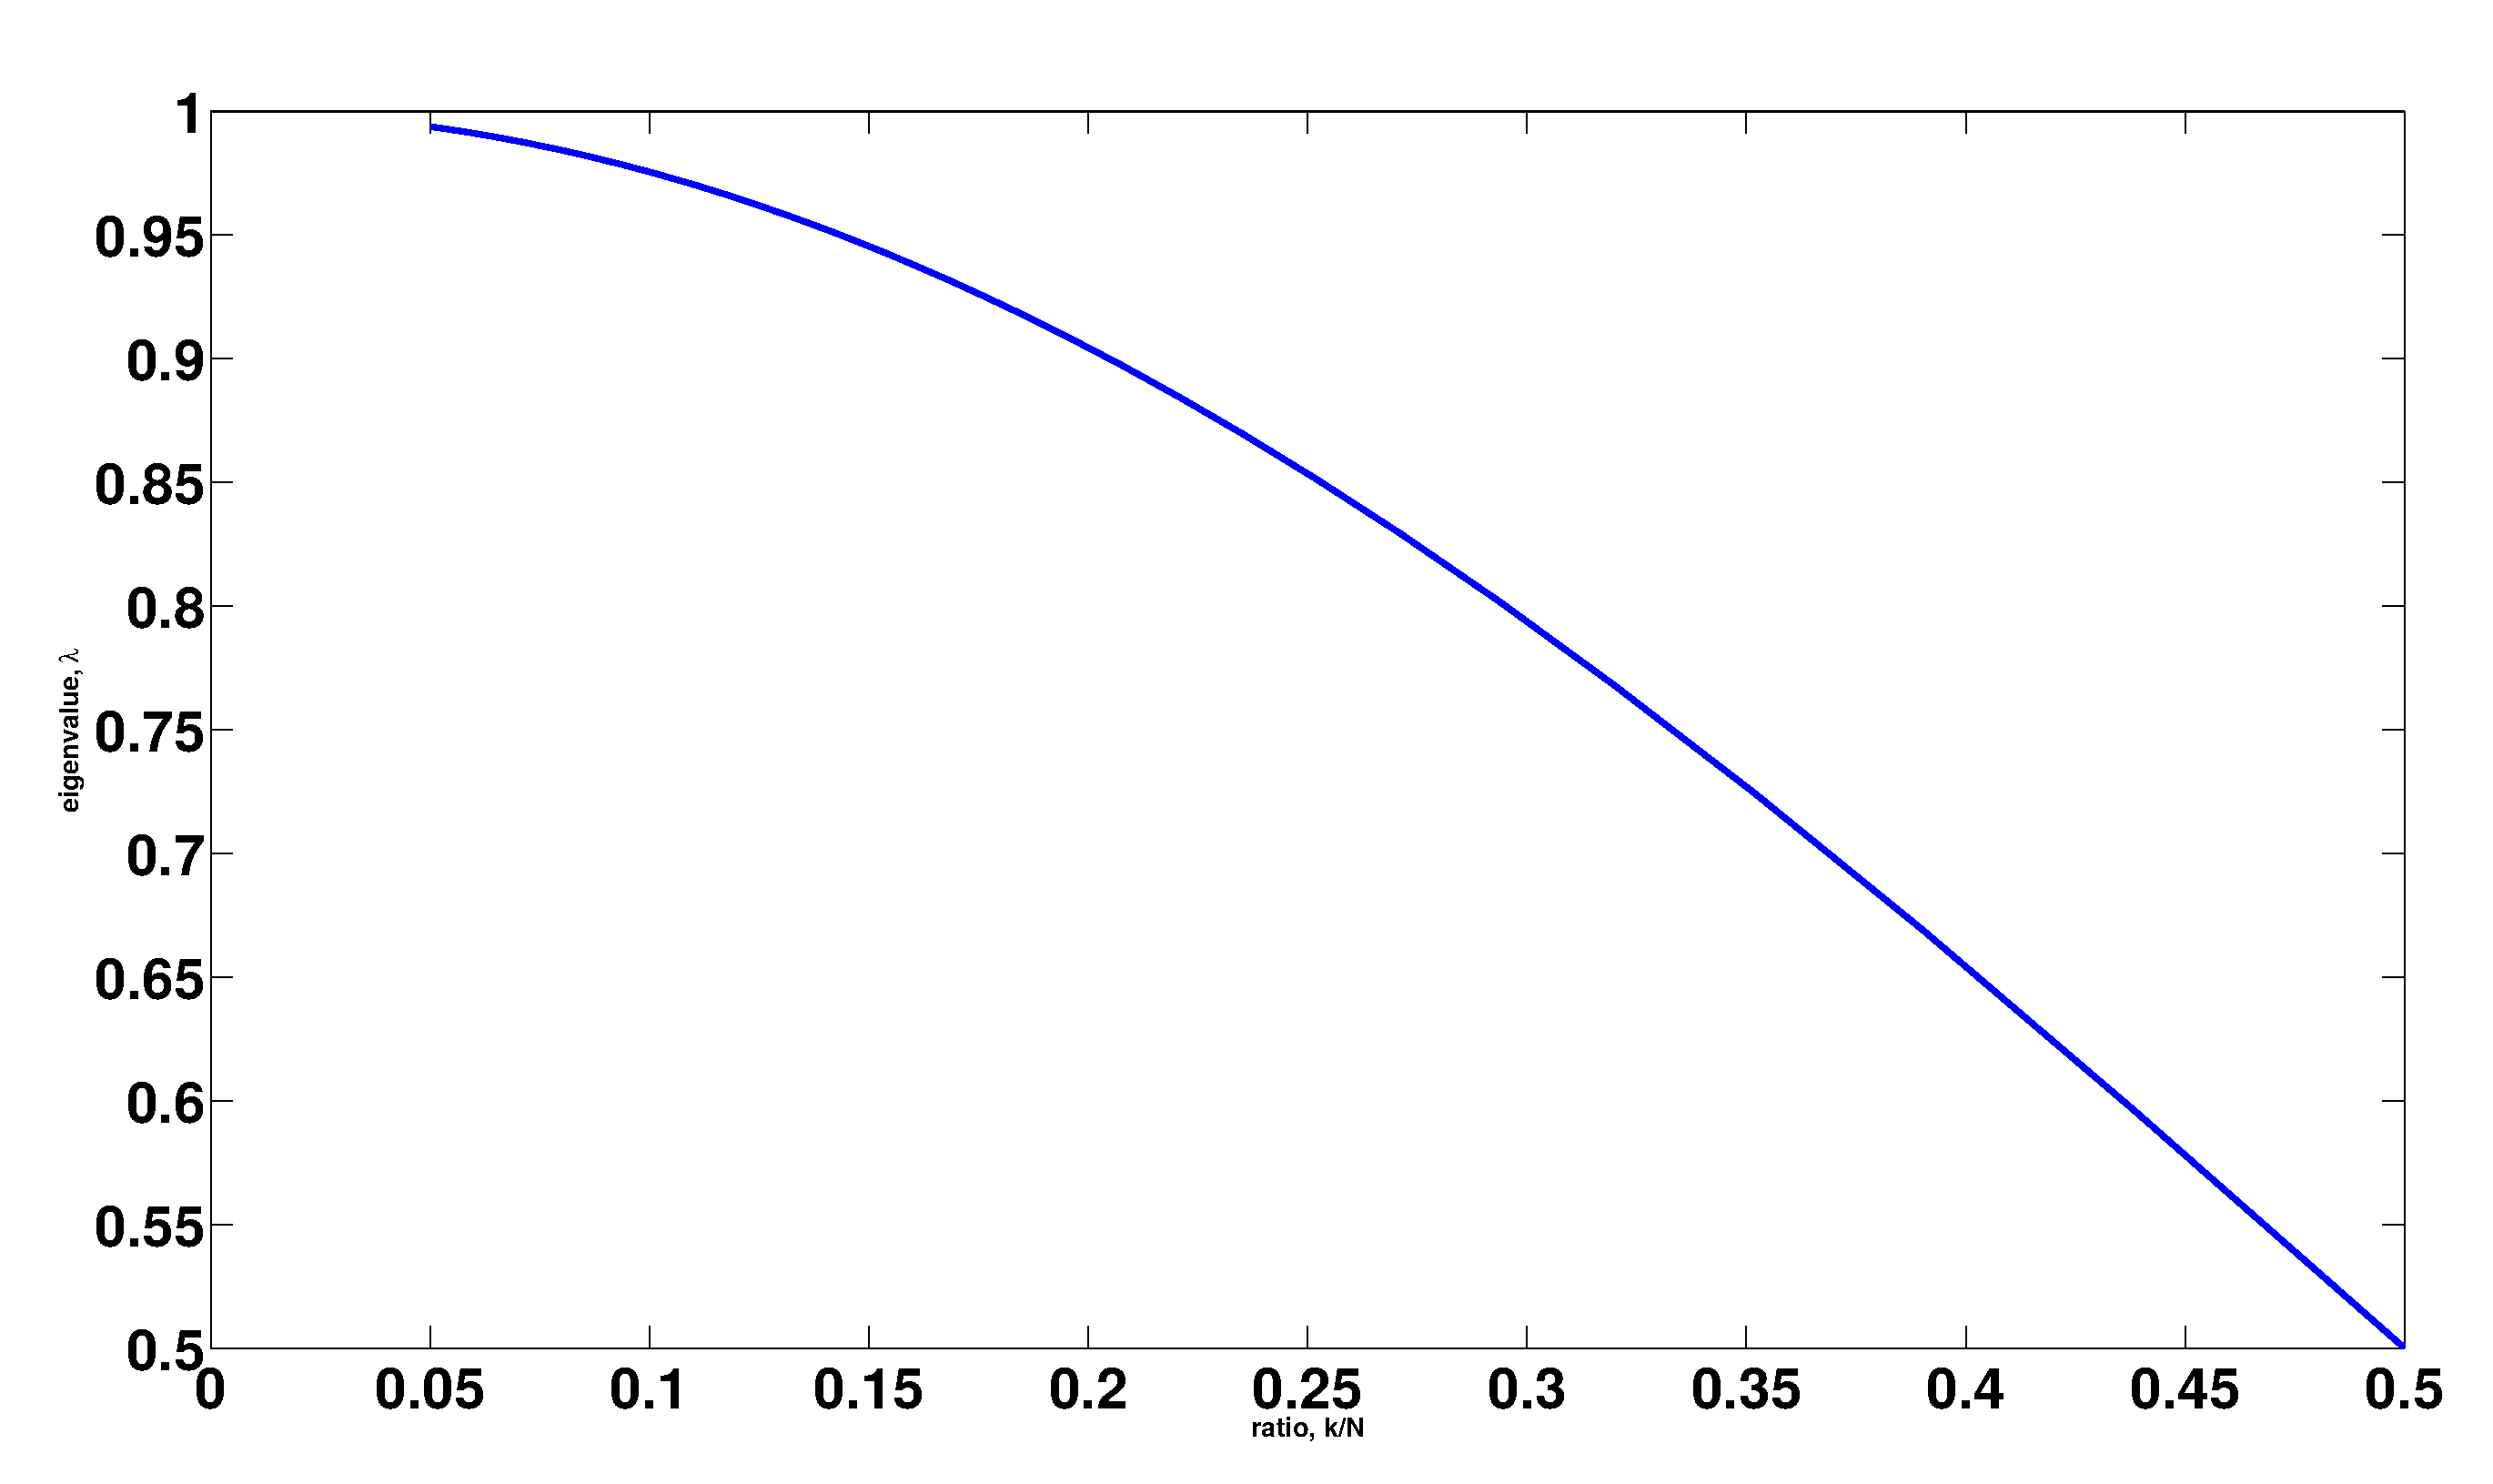
\includegraphics[scale=0.2]{eigen_vs_k-N.eps}
 \caption{Eigenvalues$\lambda$ with respect to $\frac{k}{N}$}
 \label{Fig:eig_vs_k-N}
\end{figure}

\begin{figure}
 \centering
 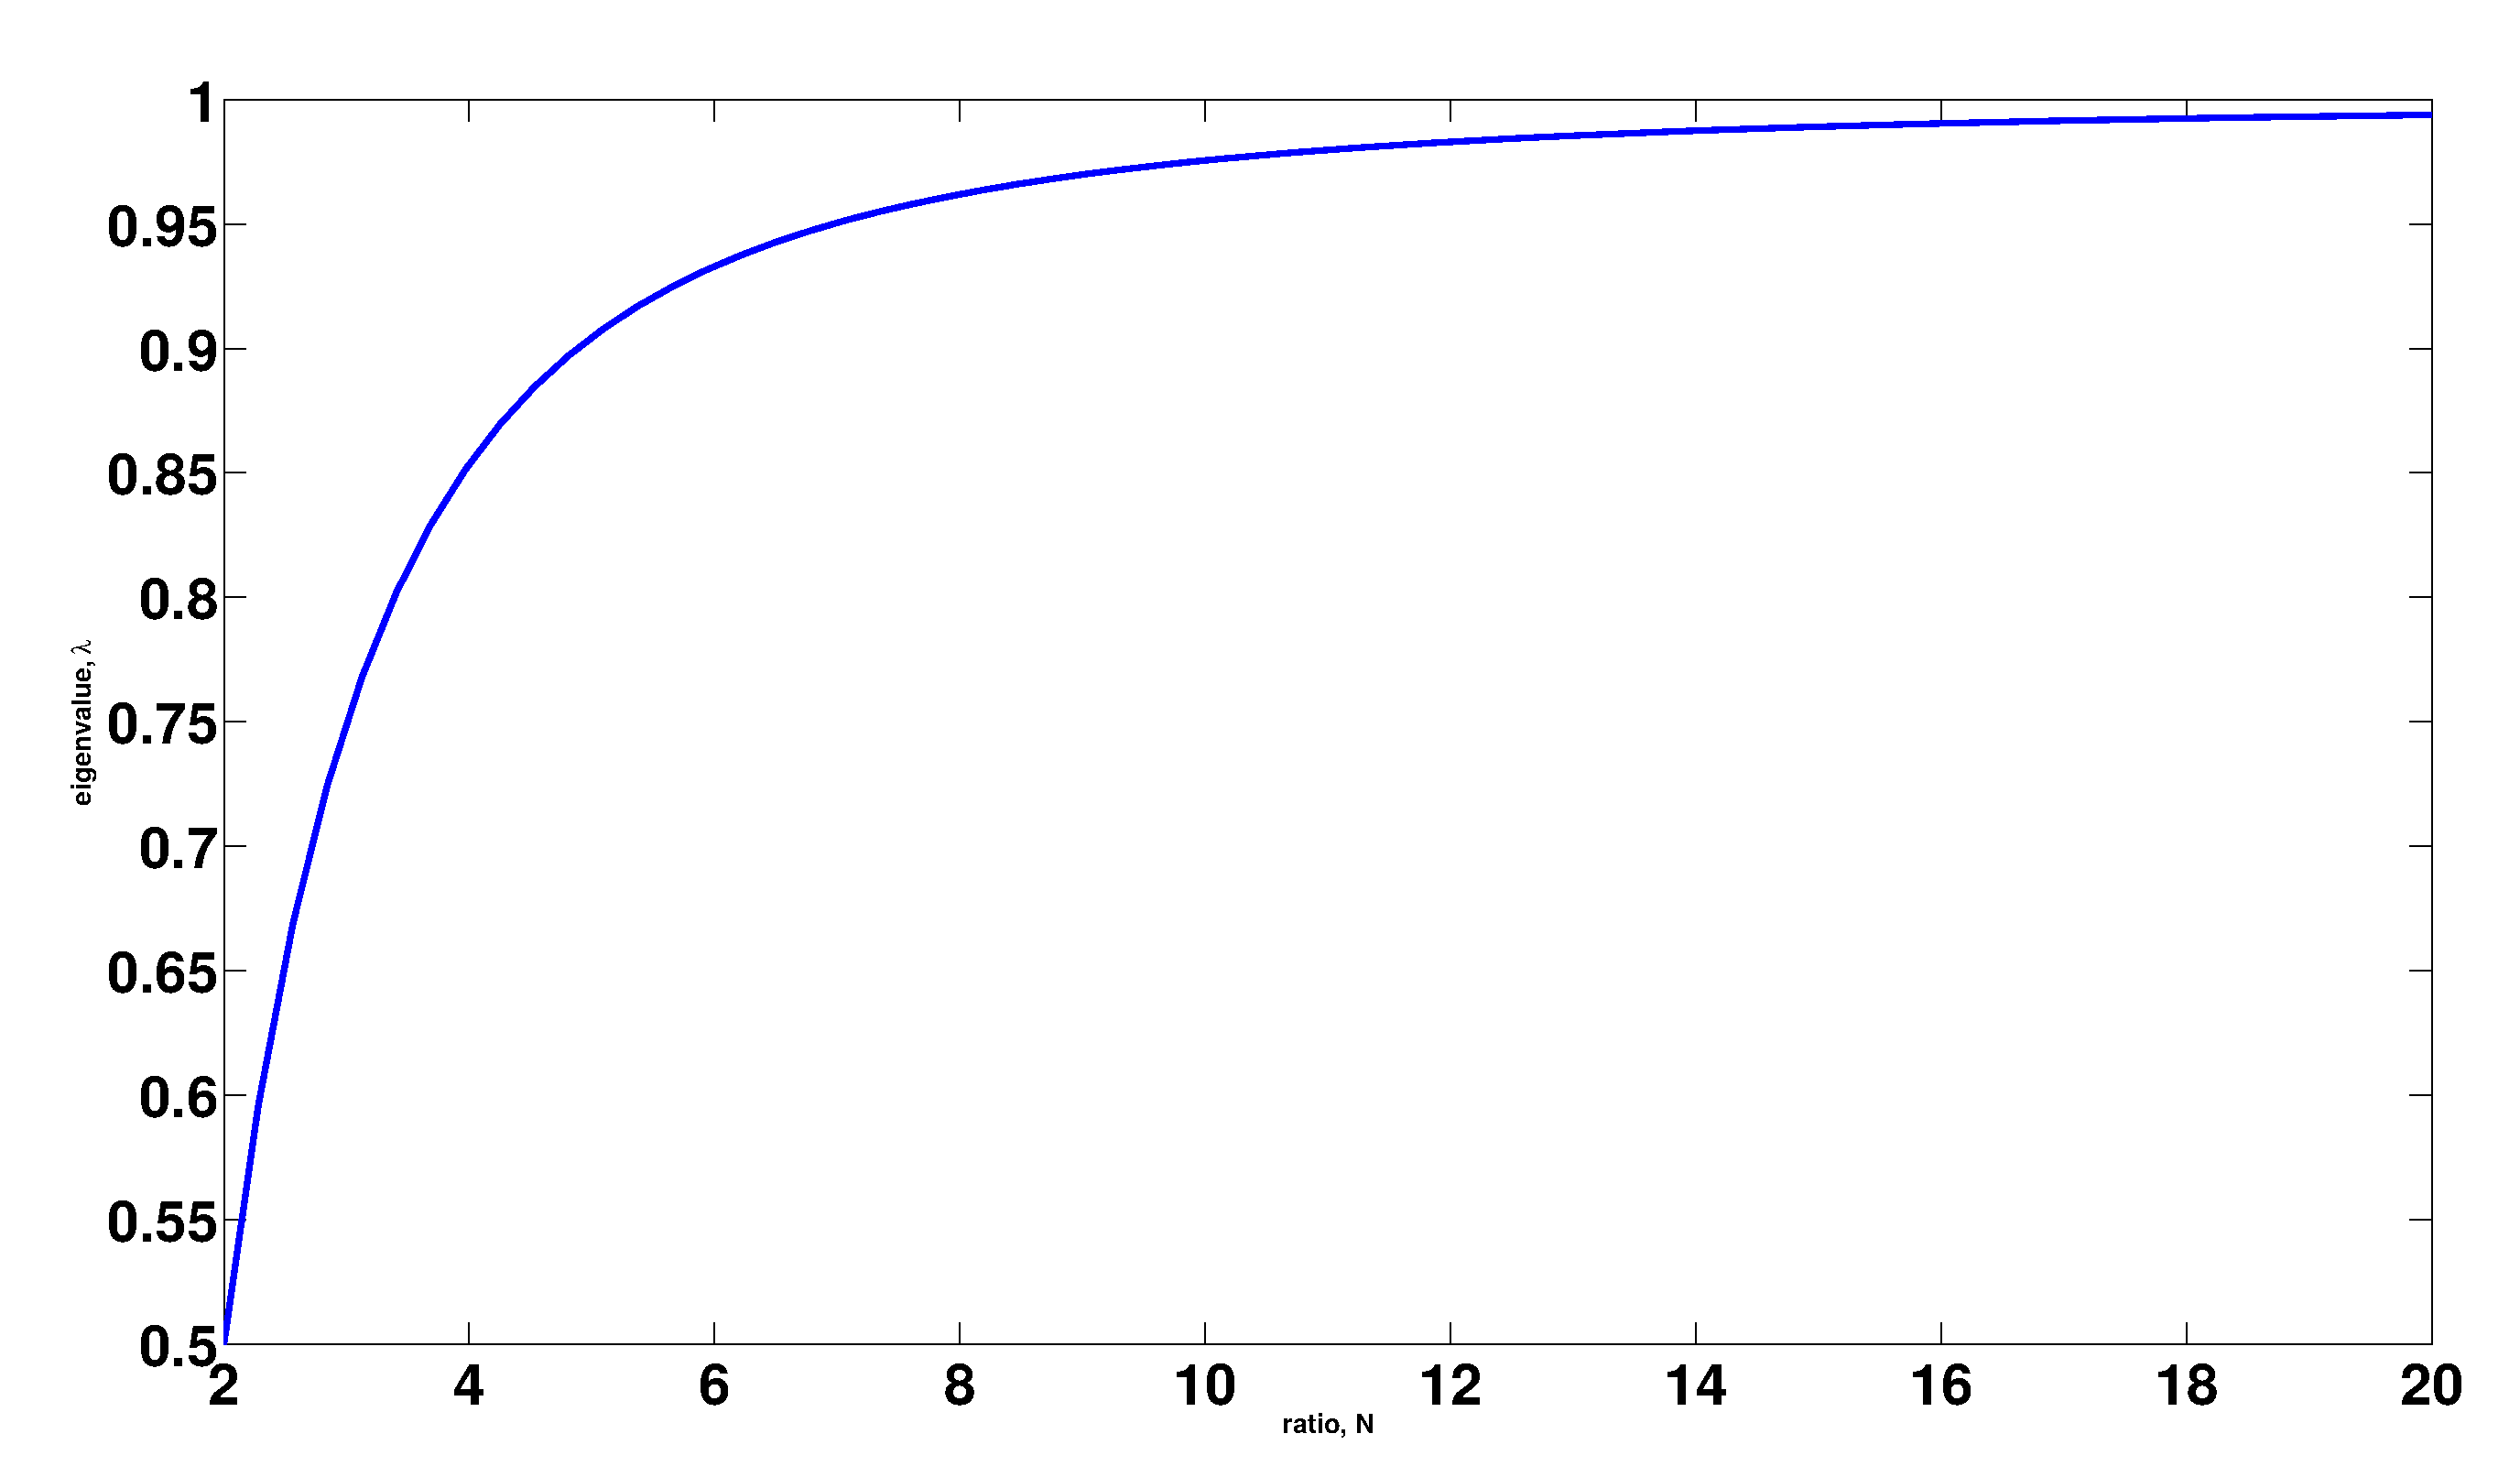
\includegraphics[scale=0.2]{eigen_vs_N.eps}
 \caption{Eigenvalues$\lambda$ with respect to N}
 \label{Fig:eig_vs_N}
\end{figure}


\section{Algorithm of Multigrid method}

In the light of above results, we can think of an strategy to exploit the faster convergence characteristics of the method. It could be to solve the problem on 
coarser grids and interpolate the result on finer grid. This would be a better guess for finer grid and we can repeat the process till the finest grid when we 
want the solution. 
The disadvantages of this strategy are:
\begin{enumerate}
 \item The problem is solved fully on coarser grids even we are only interested in the solution on finest grid.
 \item It does not make use of any guess which we can have from finer grids.
 \item Sometimes the problem is not well resolved on coarser grids and hence the guess provided by the coarser grid solution might not be a good guess.
\end{enumerate}

A better strategy is to coarse grid correction, which calculates the error on coarser grids and provide a correction on the finest grid. We have defined the 
error as:
\begin{equation}
 \begin{align}
  \text{exact solution} \quad Ax^e &= b \\
  \text{solution at k\textsuperscript{th} iteration} \quad Ax^k &= b -r \\
  \text{error at k\textsuperscript{th} iteration} \quad e^k &= x^e - x^k \\
  \text{from above, we get,}\quad A(x^e-x^k) &= r \\
  \text{or,} \quad  Ae^k &= r
 \end{align}
 \label{E7}
\end{equation}

We solve the given problem $Ax = b$ on the finest grid, and $A^e = r$ on the coarser grids. The basic steps in the algorithm are:
\begin{enumerate}
 \item Iterate for few steps the given problem on the finest grid. This step is \textbf{relaxation}. 
 \item Transfer the residue from finest grid to coarser grid. This step is called as \textbf{restriction}.
  \item Interpolate the values of error and add it previous values to make a correction. This step is
    \textbf{prolongation}.
\end{enumerate}

The algorithm for multigrid is followed as in Fig. \ref{Fig:fd_mg}. This is V cycle algorithm, where the restriction is done till the coarsest grid and then prolongation till 
the finest grid.% (See Fig \ref{Fig:Vcycle}). put a V figure for vcycle later.
\begin{figure}
 \centering
 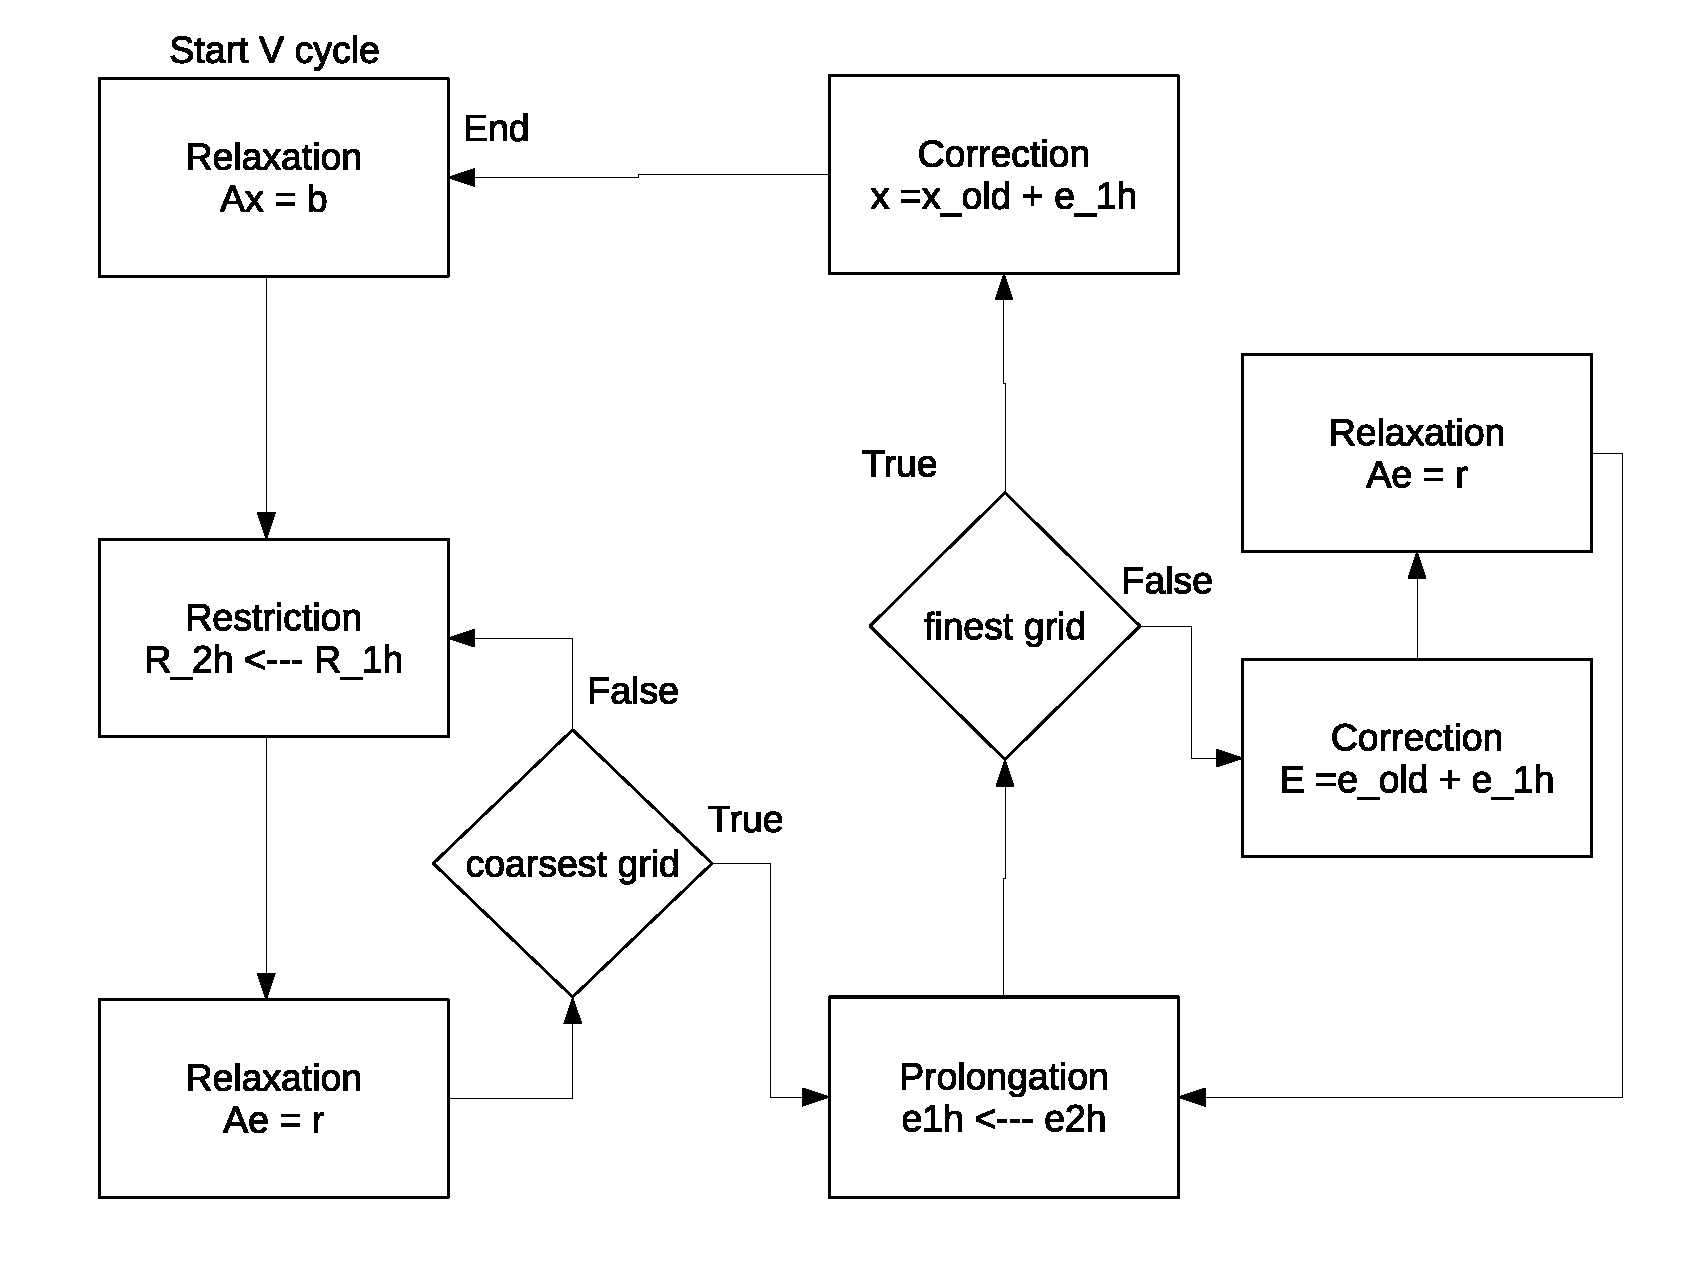
\includegraphics[scale=0.5]{fd_mg.eps}
 \caption{Multigrid Algorithm}
 \label{Fig:fd_mg}
\end{figure}

\section{Sample Problem}

We try to solve to some problems to understand the implementation details of the algorithm. Consider a one dimensional Poisson's equation \ref{E8},
\subsection{One dimensional Poisson's equation}
\begin{equation}
 \frac{d^2 u}{dx^2} = \frac{1}{2}[sin \pi x + sin 16 \pi x]
 \label{E8}
\end{equation}

having boundary conditions $u(0) = u(1) = 0$. We can discretise Eq. \ref{E7} as,

\begin{equation}
 \frac{u_{i+1}-2u_{i}+u_{i-1}}{h^2} = \frac{1}{2}[sin \pi x_i + sin 16 \pi x_i]  
 \label{E9}
\end{equation}

Let the RHS be $q_i$ at i\textsuperscript{th} node. Then we can write for $u_i$ from \ref{E9} as,

\begin{equation}
 u_i^{n+1} = \frac{1}{2}(u_{i+1}^n+u_{i-1}^{n+1}-h^2 q_i)
 \label{E10}
\end{equation}

%Eq. \ref{E10} can be solved using Gauss-Sidel method where we can see the residue at n\textsuperscript{th} iteration in Fig. \ref{Fig:GS}. 

Eq. \ref{E10} is iteration equation for Gauss-Sidel method but for multigrid we iterate only few times. Here we will iterate only once in 
each step in a V-cycle. We have the finest grid having N = 64 with total nodes N + 1 i.e. 65. We now restrict the residue to the coarser
grid which has N/2+1 nodes. We can use average restriction as, 

\begin{equation}
 r^{2h}_i = \frac{1}{4} (r^h_{2i-1} + 2r^h_{2i} + r^h_{2i+1})
 \label{E11}
\end{equation}

Then iterate for error on the coarser grid as,

\begin{equation}
 e_i^{n+1} = \frac{1}{2}(e_{i+1}^n+e_{i-1}^{n+1}-h^2 r_i)
 \label{E12}
\end{equation}

restriction and iteration continues till the coarsest grid. At coarsest grid the iteration the error equation is solved exactly. Then the 
error is interpolated backwards for prolongation step as,

\begin{equation}
\begin{align}
 e^{h}_i &=& e^{2h}_i \quad \text{i = 0,...,N}\\
  e^{h}_{2i+1} &=& \frac{e^{2h}_i +  e^{2h}_{i+1}}{2} \quad \text{i=0,...,N}
 \end{align}
 \label{E11}
\end{equation}

While prolongation iteration step is taken at every grid level and at finest grid, we add the interpolated error to the $u$, again start with 
the V-cycle with the new $u$ as a guess. The results for this problem are compared with \cite{moin2010fundamentals} (See Fig. \ref{Fig:moin1D}).

\begin{figure}
 \centering
 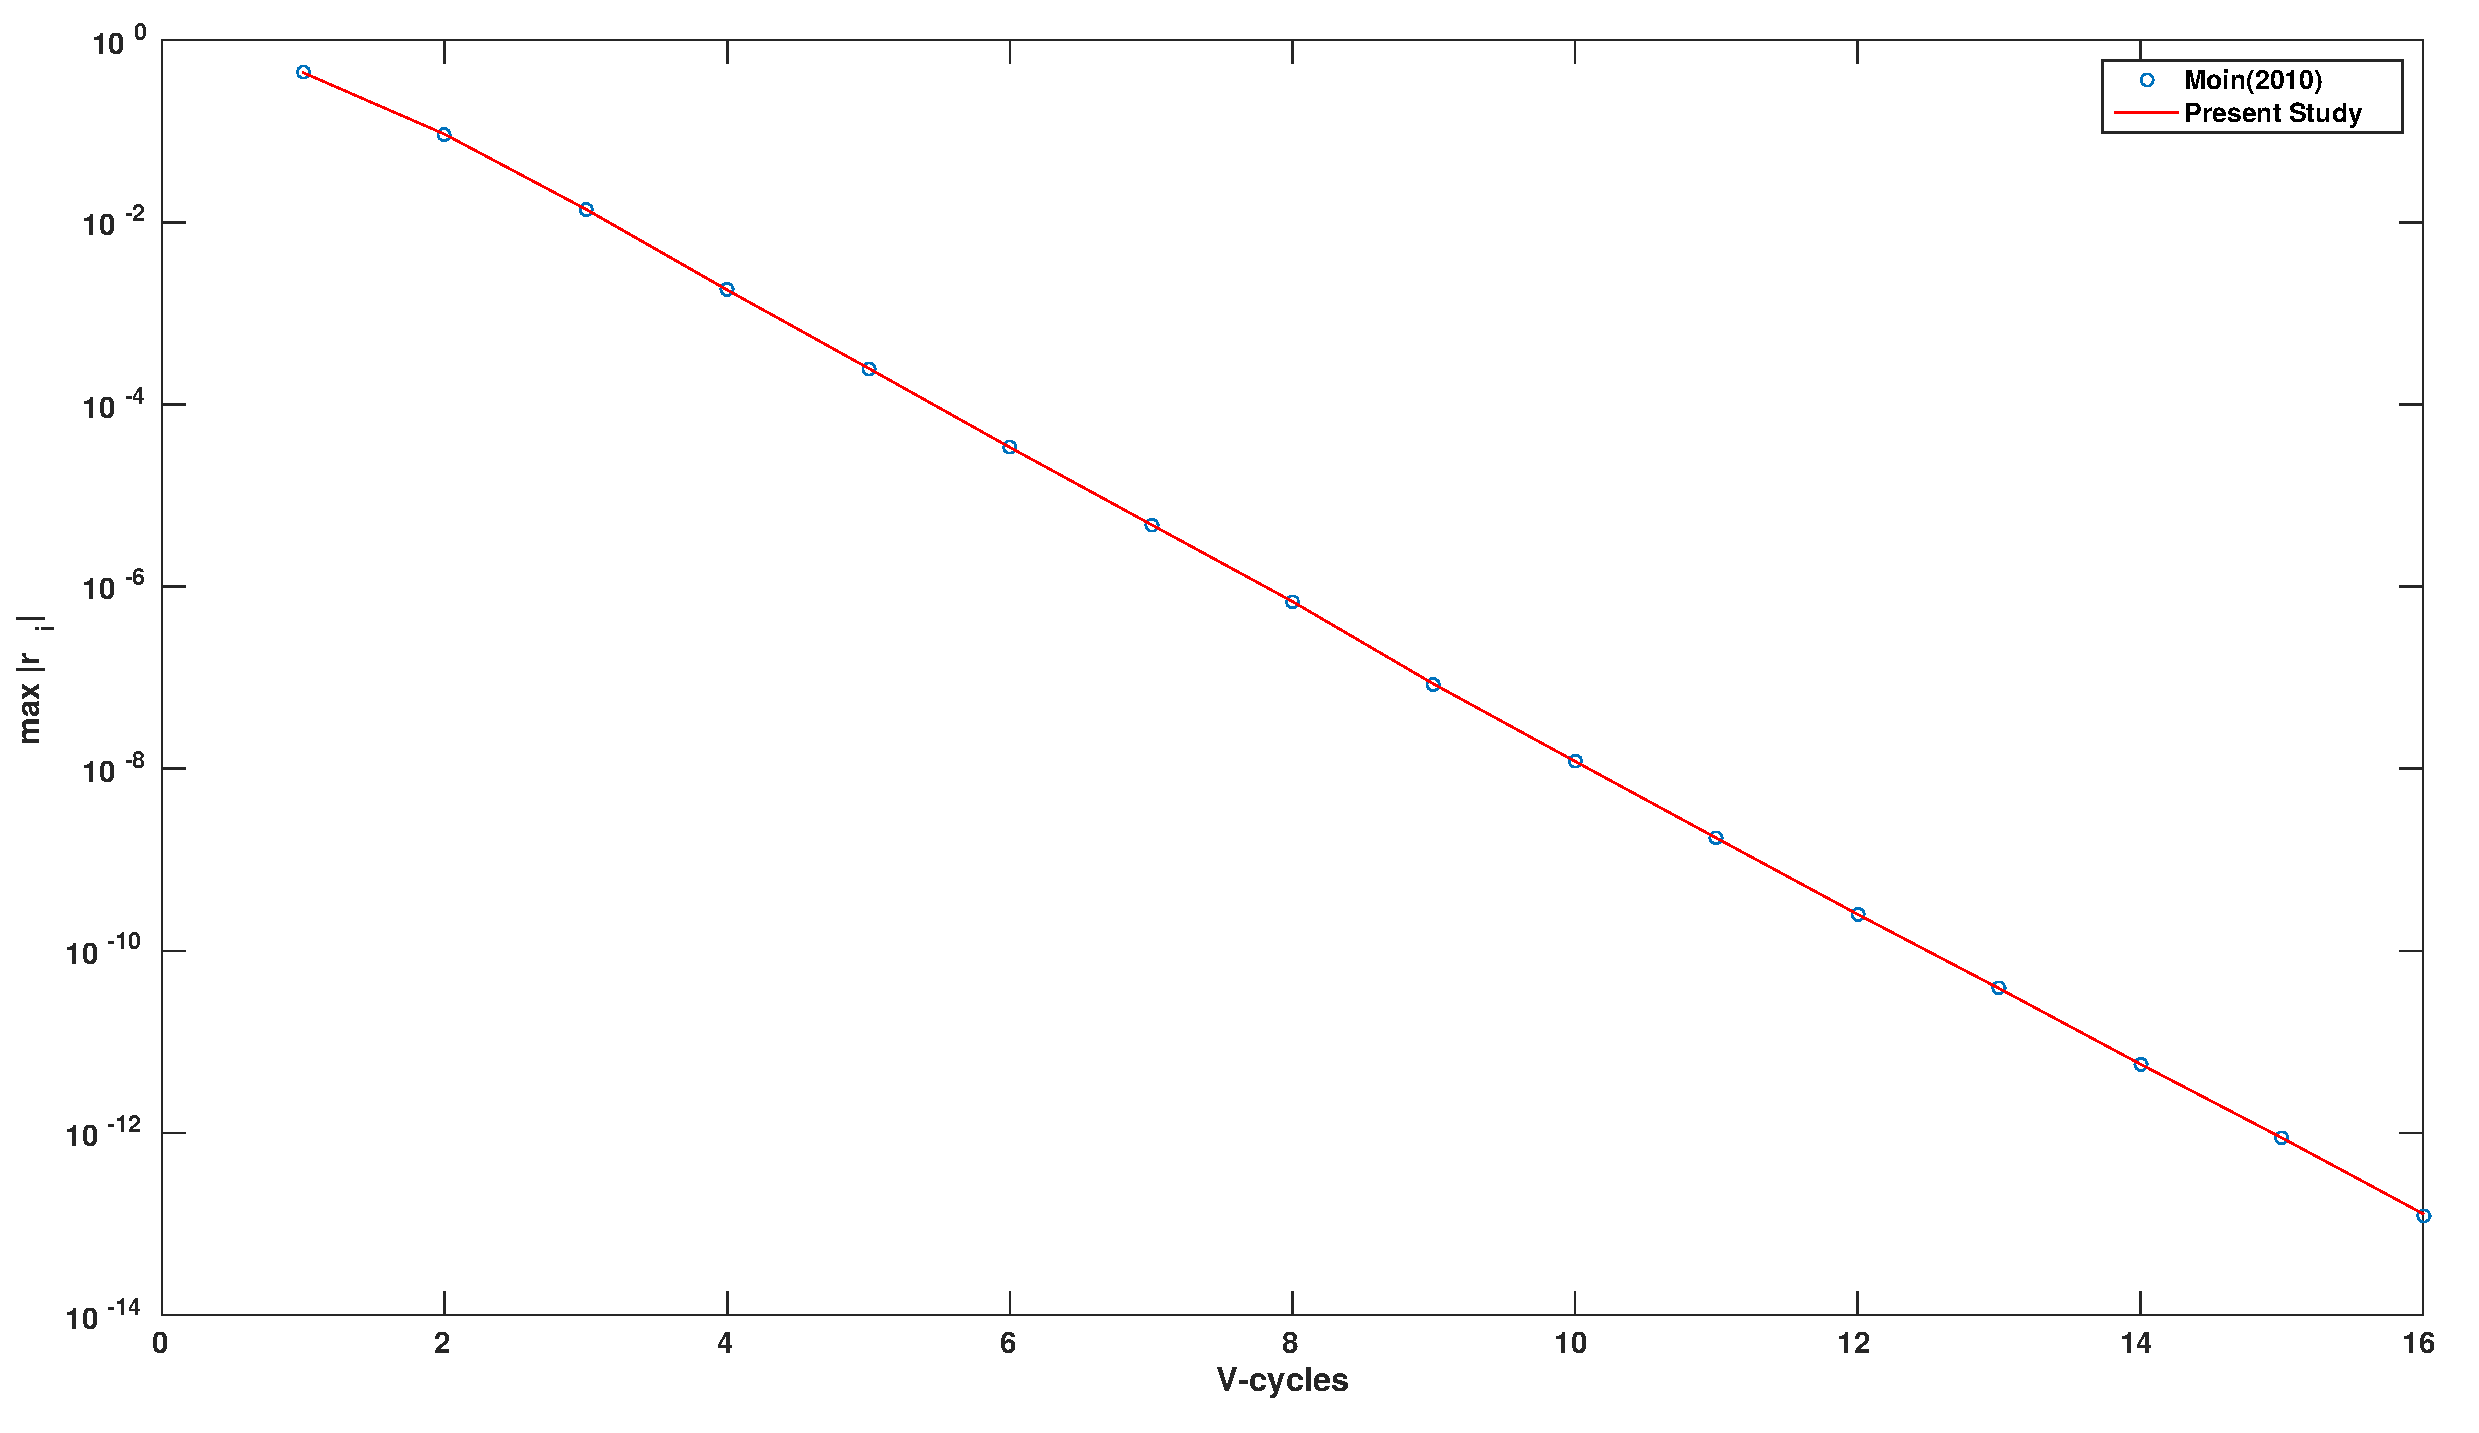
\includegraphics[scale=0.4]{moin_1D.eps}
 \caption{Comparison with Moin(2010)}
 \label{Fig:moin1D}
\end{figure}

\subsection{Two dimensional Poisson's equation}

We are interested in solving the Poisson equation, Equation \ref{eq:Poisson}, in a square domain of size unity centered on
unity with Neumann boundary conditions on all sides (\cite{Popinet2003}).

\begin{equation}
{\nabla}^2 \phi = f(x,y)
\label{eq:Poisson}
\end{equation}

\noindent Source term $f(x,y)$ is given by

\begin{equation}
f(x,y) = -{\pi}^2(k^2+l^2)\sin(\pi k x)\sin(\pi l y)
\label{eq:Source}
\end{equation}

\noindent with $k=l=3$. Exact solution of the Poisson equation with this source term is

\begin{equation}
\phi(x,y) = \sin(\pi k x)\sin(\pi l y) + \kappa
\label{eq:Solution}
\end{equation}

\noindent where $\kappa$ is an arbitary constant.

\section{Discretization}

Problem domain, shown in Figure \ref{fig:discretization}, is discretized using a 2nd-order
finite difference approximation on a cartesian grid having N nodes in both x- and y-directions which correspondes
to a uniform grid spacing h. The value of $\phi$ on the 2D cartesian mesh can then be approximated
for each node {i,j} in the interior of the computational domain as

\begin{equation}
\frac{1}{h^2} \left({{\phi}^n_{i-1,j}} + {{\phi}^n_{i,j-1}} -4 {{\phi}^{n+1}_{i,j}} + {{\phi}^n_{i+1,j}} + {{\phi}^n_{i,j+1}} \right) = f_{i,j}, \hspace{1 cm} i, j = 2,..., N-1
\label{eq:discretization}
\end{equation}

\noindent where the subscripts $i$ and $j$ represent the indices of the current node in the computational domain for the
$x$ and $y$ directions, respectively.

\begin{figure}
\begin{center}
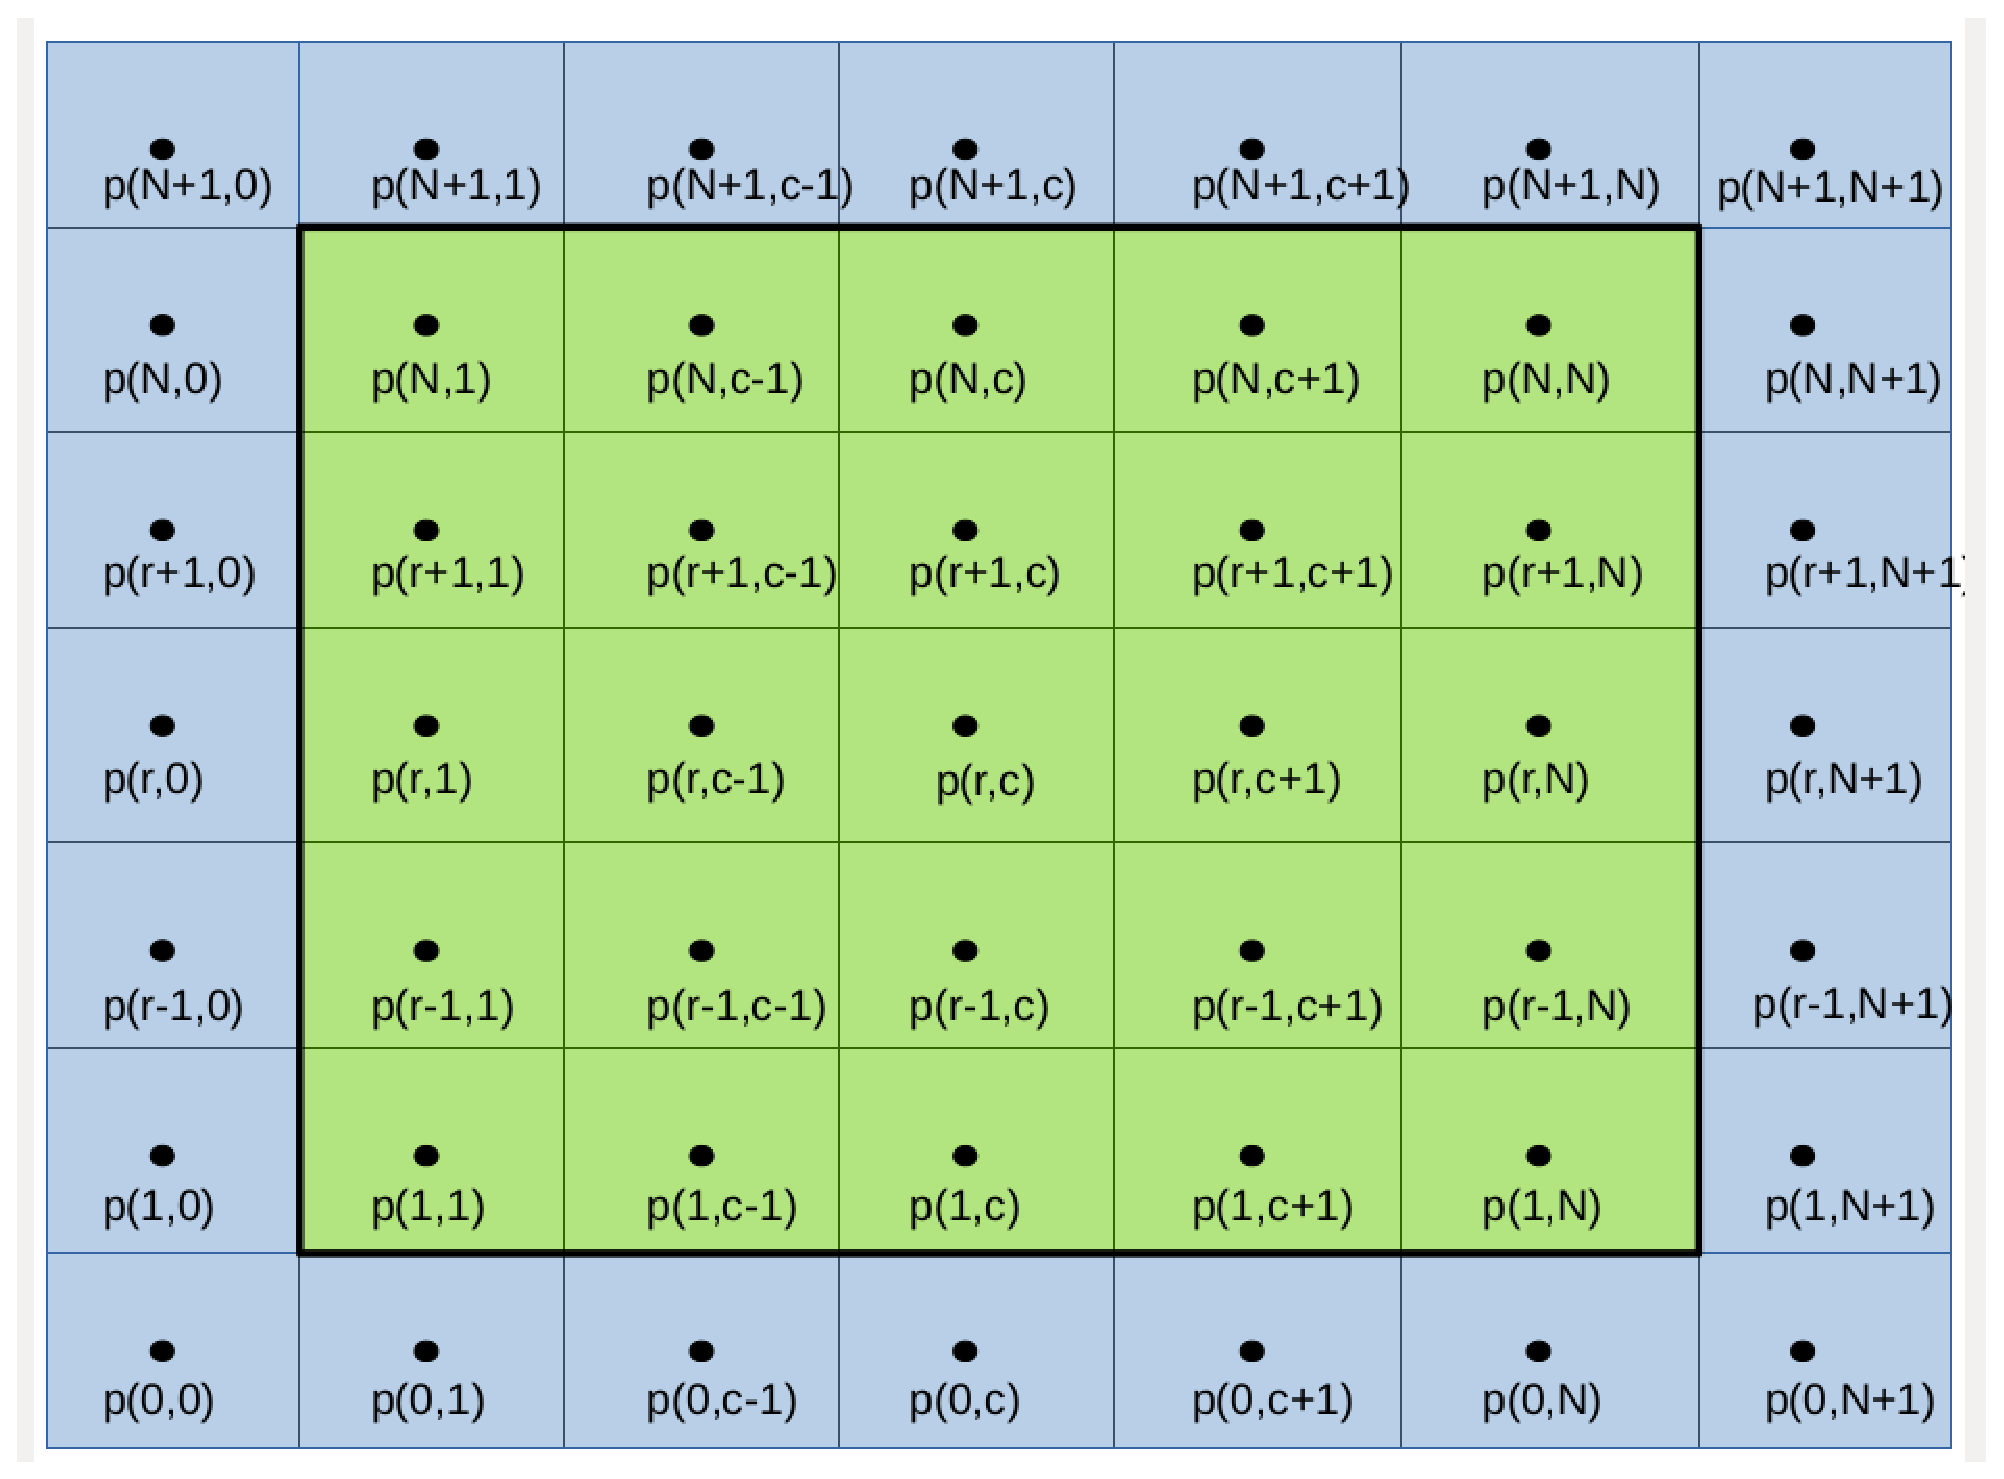
\includegraphics[width=3.0 in]{pressure.eps}
\end{center}
\caption{2D uniform mesh featuring a discretization with a 5-point stencil.}
\label{fig:discretization} 
\end{figure}

\section{Validation}

\begin{figure}
\begin{center}
{\tiny
\begin{tabular}{cc}
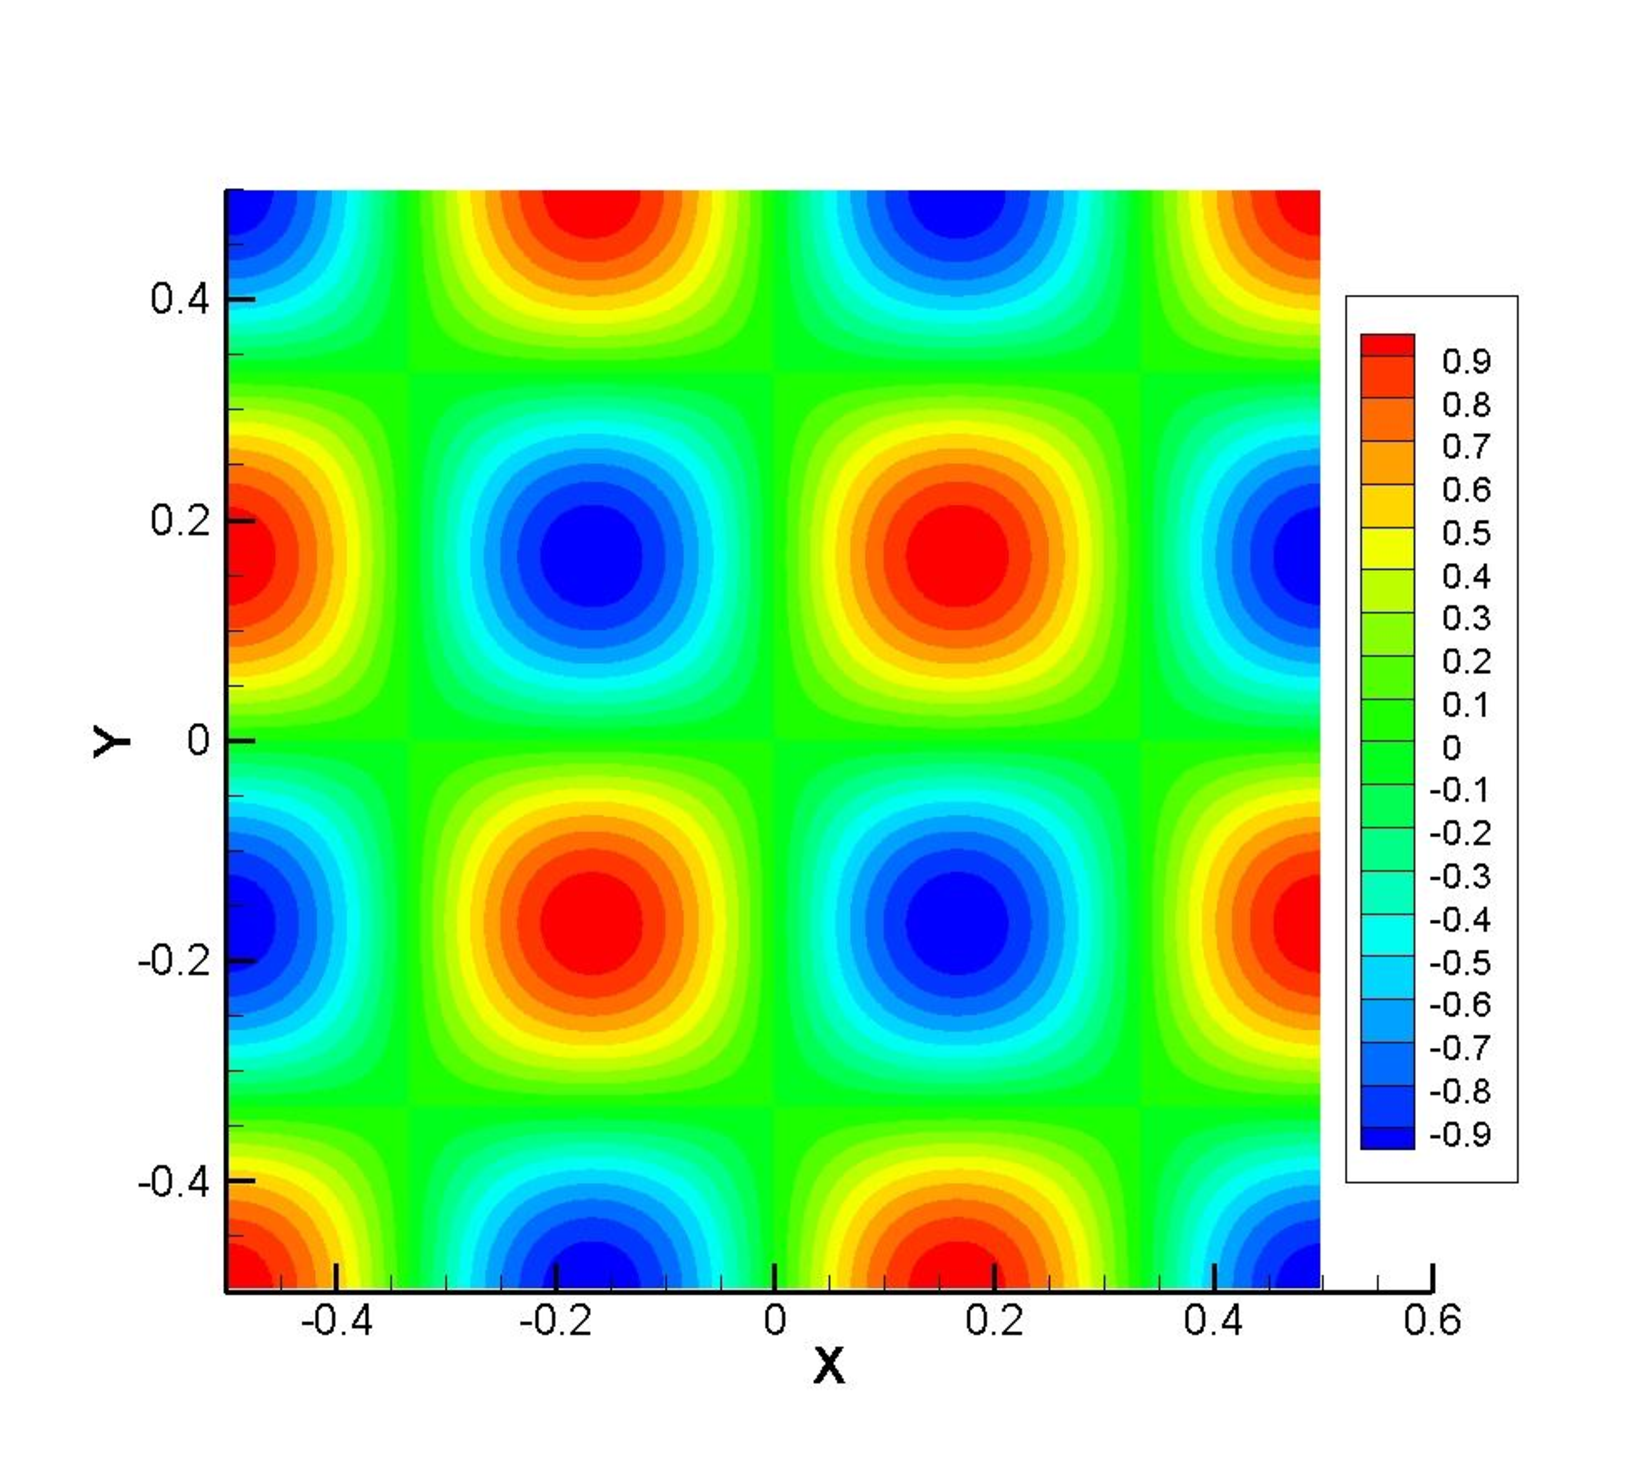
\includegraphics[width=4.0in]{sol_N500_np1.eps} \\
(a) \\
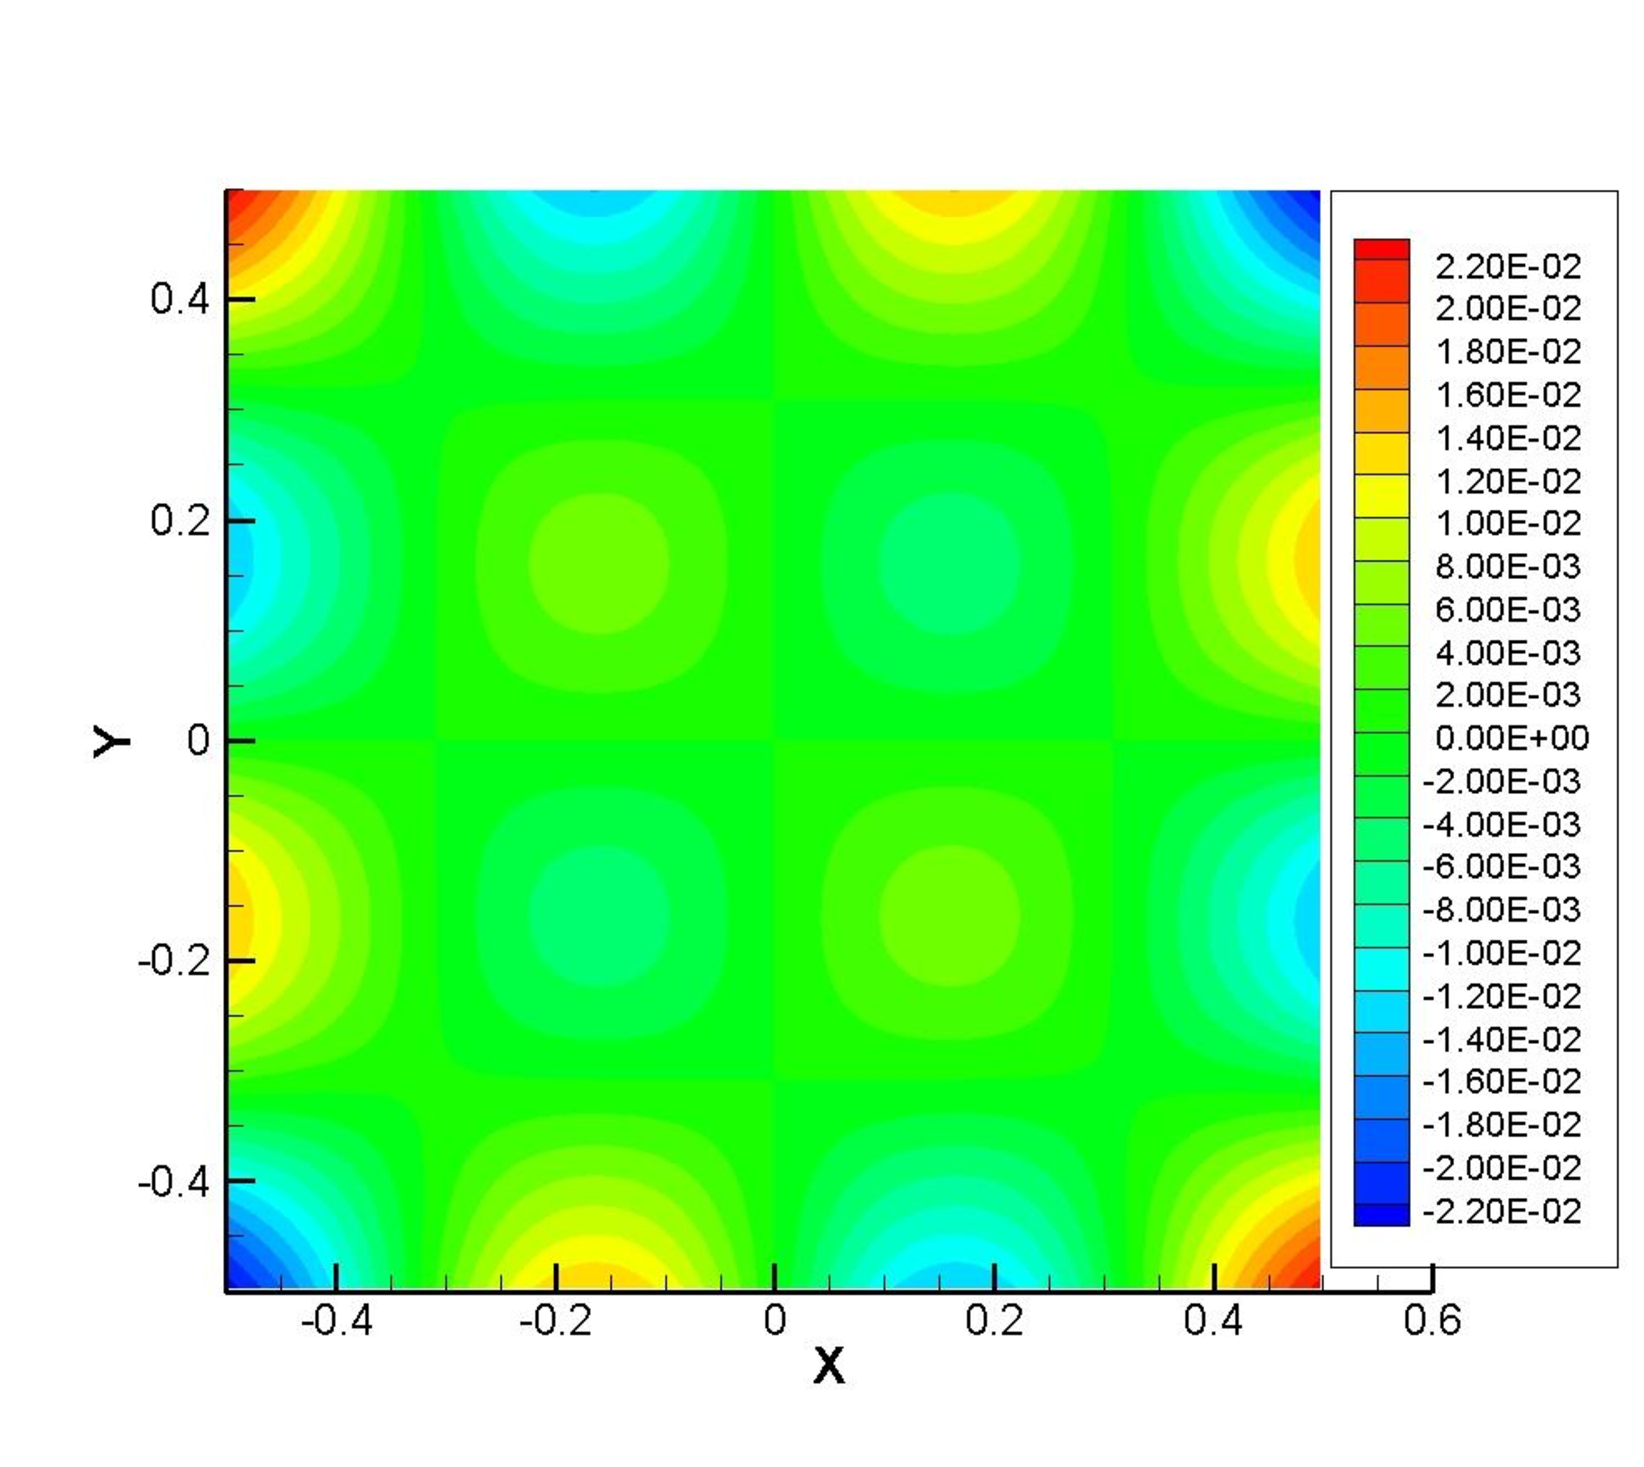
\includegraphics[width=4.0in]{err_N500_np1.eps} \\
(b)
\end{tabular}}
\end{center}

\caption{Solver results of for $N=500$ and $np=4$; (a) Poisson solution and (b) solution error.}
\label{fig:dsmc_cfd1}
\end{figure}
\newpage
\section{Comparison with SOR Parallel}
The same problem is solved using SOR (MPI) and the results are compared.

The following tests performed on the a machine having the following specifications:

\begin{enumerate}
 \item Processor:  Intel(R) Xeon(R) CPU E5-1650 v3 @ 3.50GHz
 \item CPU Cores: 6 (6 more with hyperthread-Virtual cores)
 \item RAM:	 64 GB
 \item Cache:    15360 KB
\end{enumerate}

\begin{figure}
\begin{center}
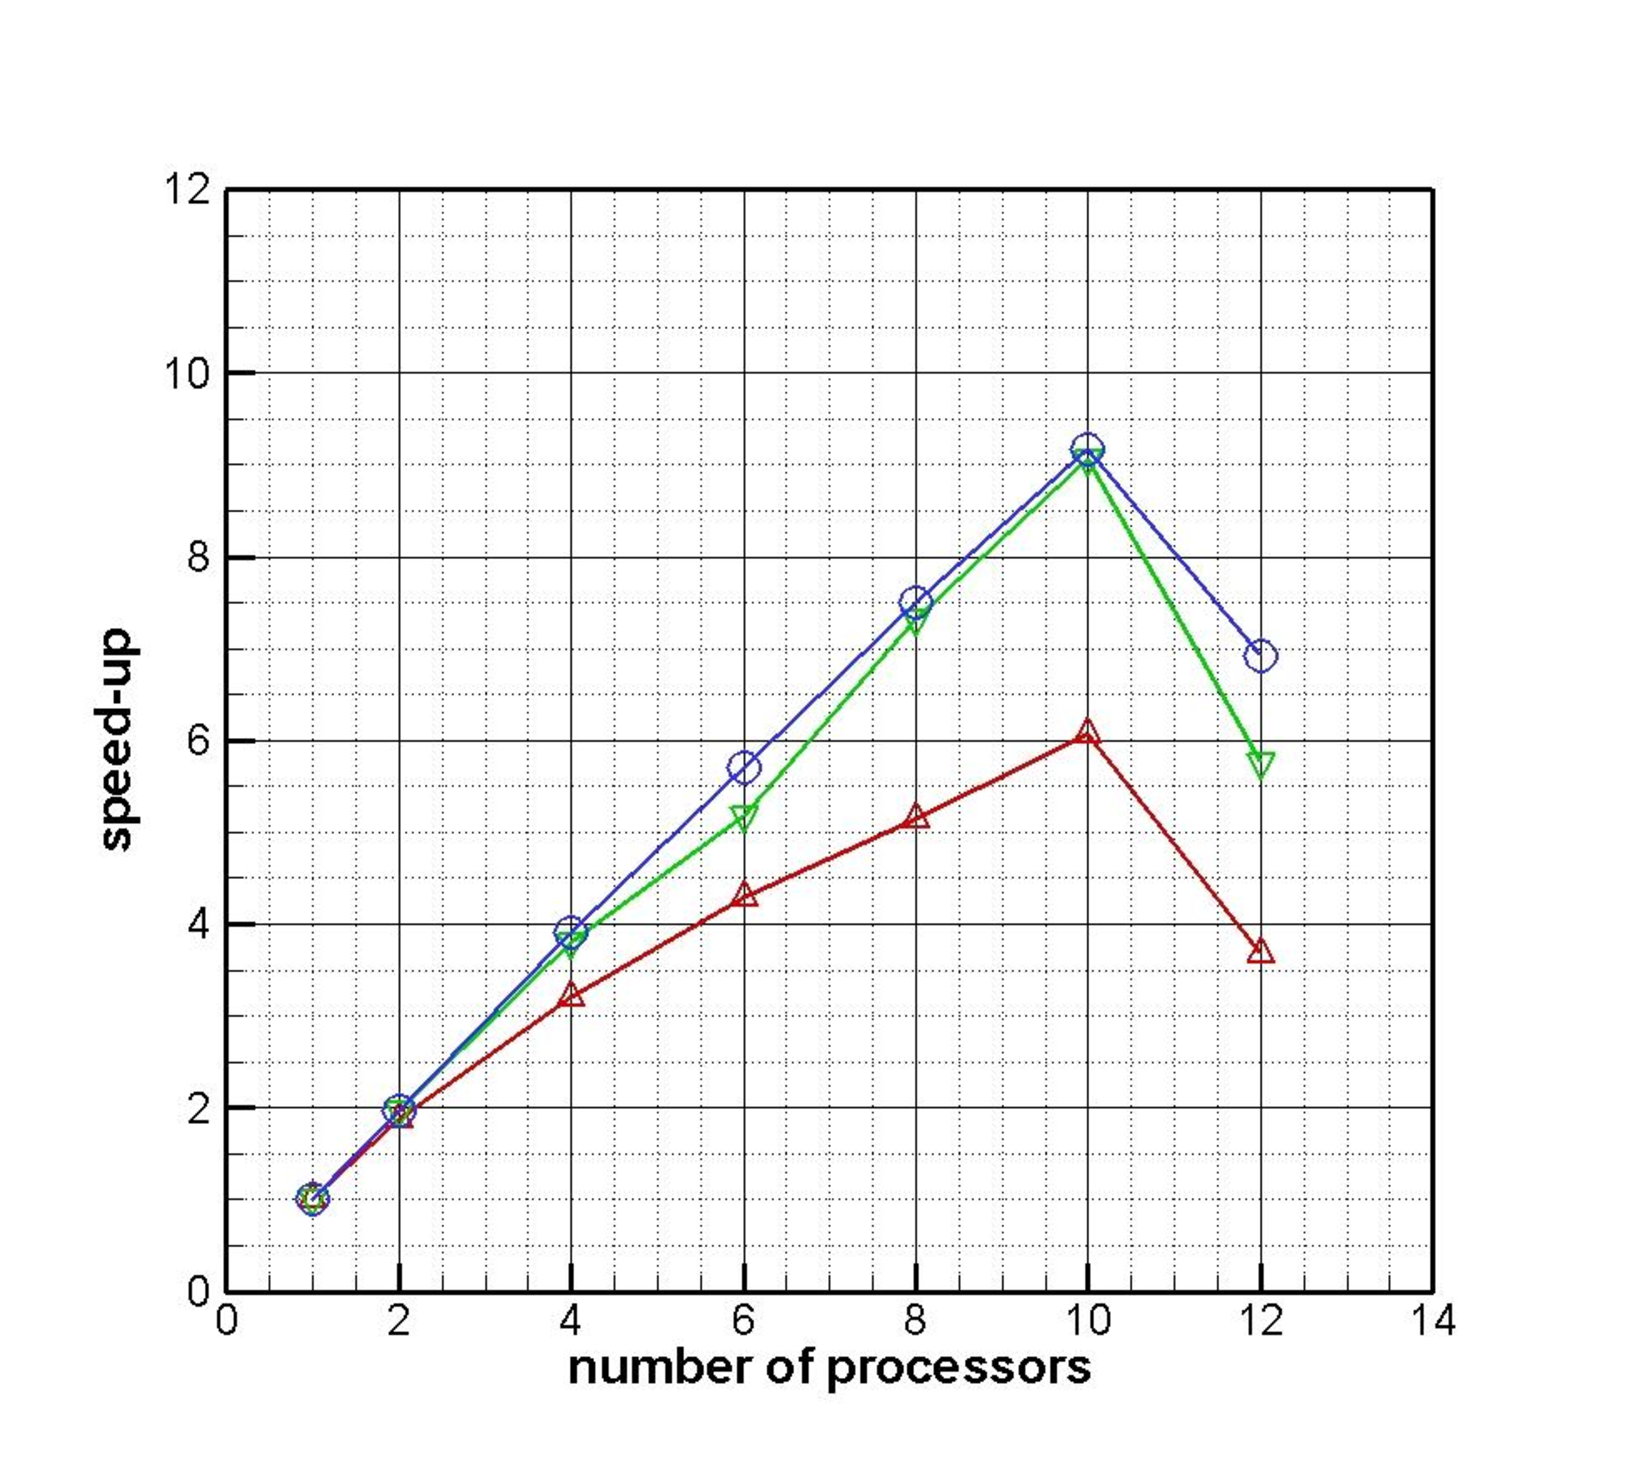
\includegraphics[width=5.0 in]{speedup.eps}
\end{center}
\caption{Speedup values for MPI parallel (SOR) Poisson equation solver.}
\label{speedup} 
\end{figure}

\begin{figure}
\centering
 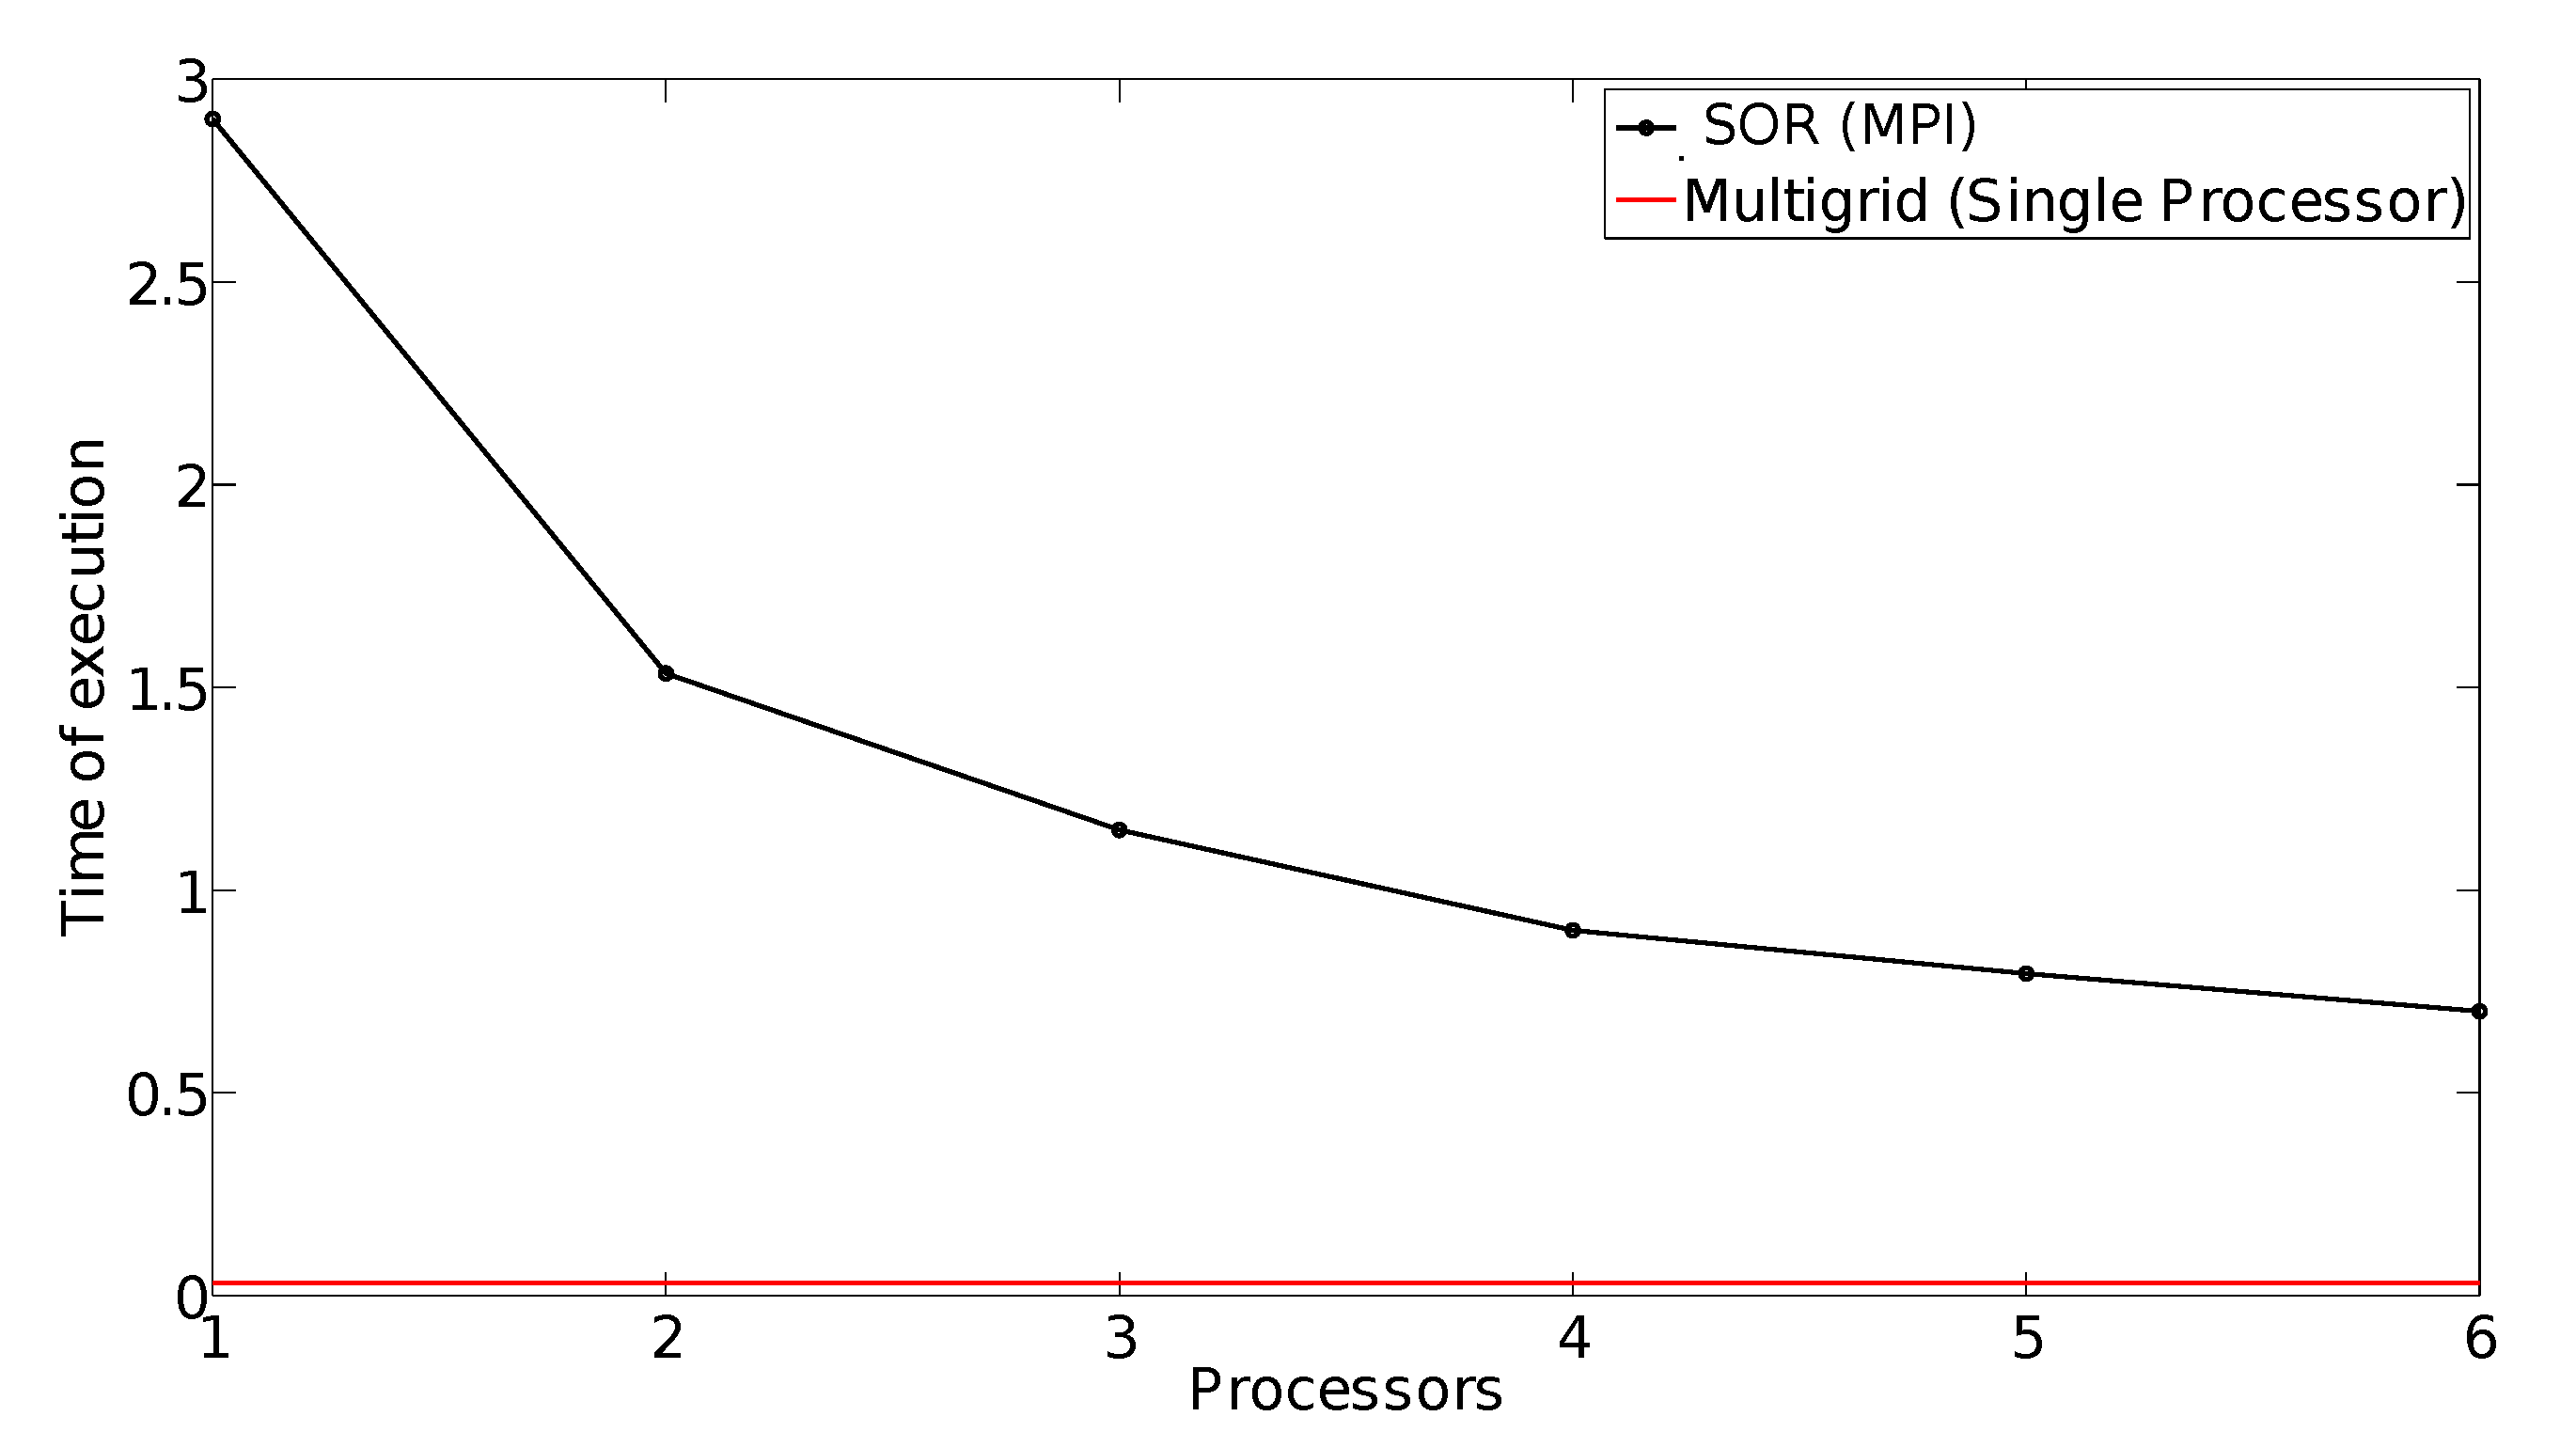
\includegraphics[scale=0.25]{comparison.eps} 
 \caption{Comparison of SOR and Multigrid Time of execution}
 \label{comparison_mg}
\end{figure}

From Fig.\ref{speedup} it can be observed that time of execution has decreased with increase in number of processors and speed up is more 
for larger size problem. A decrease in speed up is seen when the number of processors were more than the physcial cores and the threads took
more time to process. Fig. \ref{comparison_mg} has emphasizes the fact that multigrid on a single processor is far more efficient on a multicore
SOR algorithm. Hence this work can be further extended for parallelizing the multigrid algorithm.















